\documentclass[12pt]{report}
\usepackage[fontsize=13pt]{scrextend}
\usepackage[utf8]{vietnam}
\usepackage[utf8]{inputenc}
\usepackage[vietnamese]{babel}
\usepackage{titlesec}
\usepackage{titletoc}
\usepackage{listings}
\usepackage[bookmarks=true]{hyperref}
\usepackage[left=3cm,right=2cm,top=2.5cm,bottom=3cm]{geometry}
\usepackage{graphicx}
\usepackage{hyperref}
\usepackage{tikz}
\usepackage{varwidth}
\usepackage{float}
\usepackage{color}
\usepackage{multirow}
\usepackage{booktabs}
\usepackage[ruled,vlined]{algorithm2e}
\usepackage{chngcntr}
\usepackage{nameref}
\usepackage{calc}
\usepackage{svg}
%\usepackage[font=bf]{caption}
%\counterwithin{figure}{chapter}

%\renewcommand\labelitemi{--}

\setlength{\parskip}{6pt}

\usetikzlibrary{calc}
\setlength{\parindent}{10mm}
\renewcommand{\baselinestretch}{1.3}
\graphicspath{{images/}}

%%% The following lines add Chapter or Appendix in front of the number
\titlecontents{chapter}%
[0pt]%
{\vspace{1ex}}%
{\bfseries Chương \thecontentslabel\quad}%
{\bfseries}%
{\bfseries\hfill\contentspage}
%%% Initially, for the main part of the document, set the label to "Chapter"
\let\chapappname\chaptername

\definecolor{dkgreen}{rgb}{0,0.6,0}
\definecolor{gray}{rgb}{0.5,0.5,0.5}
\definecolor{mauve}{rgb}{0.58,0,0.82}

% setup code area as listings
\lstset{frame=tb,
  language=Java,
  aboveskip=3mm,
  belowskip=3mm,
  showstringspaces=false,
  columns=flexible,
  basicstyle={\small\ttfamily},
  numbers=left,
  numberstyle=\tiny\color{gray},
  keywordstyle=\color{blue},
  commentstyle=\color{dkgreen},
  stringstyle=\color{mauve},
  breaklines=true,
  breakatwhitespace=true,
  tabsize=3
}

\renewcommand{\lstlistingname}{Mã nguồn}

\newenvironment{thuattoan}[1][h]
  {\renewcommand{\algorithmcfname}{Thuật toán}
   \begin{algorithm}[#1]
  }{\end{algorithm}}

% hyper setup
\hypersetup{
	bookmarks=true,
	pdftitle={Xây dựng công cụ phát hiện sự tuân thủ mẫu thiết kế cho các dự án sử dụng Java},
	pdfauthor={Phạm Ngọc Quý}, % author
	pdfsubject={TeX and LaTeX},
	pdfkeywords={TeX, LaTeX, graphics, images}, % list of keywords
	colorlinks=false,       % false: boxed links; true: colored links
	linkcolor=black,       % color of internal links
	citecolor=black,       % color of links to bibliography
	filecolor=black,        % color of file links
	urlcolor=black,        % color of external links
	linktoc=page            % only page is linked
}

\begin{document}
\begin{titlepage}
	\center
	\begin{tikzpicture}[overlay,remember picture]
		\draw [line width=3pt,rounded corners=0pt,]
		($ (current page.north west) + (25mm,-25mm) $)
		rectangle
		($ (current page.south east) + (-15mm,25mm) $);
		\draw [line width=1pt,rounded corners=0pt]
		($ (current page.north west) + (26.5mm,-26.5mm) $)
		rectangle
		($ (current page.south east) + (-16.5mm,26.5mm) $);
	\end{tikzpicture}
	
	{\large \bfseries ĐẠI HỌC QUỐC GIA HÀ NỘI\\ TRƯỜNG ĐẠI HỌC CÔNG NGHỆ}\\[1cm]
	
\includegraphics[width=0.2\linewidth]{uet}\\[1cm]
	{\Large  \bfseries Phạm Ngọc Quý}\\[1.5cm]
	{ \LARGE \bfseries XÂY DỰNG CÔNG CỤ PHÁT HIỆN SỰ TUÂN THỦ MẪU THIẾT KẾ CHO CÁC DỰ ÁN SỬ DỤNG JAVA }\\[0.5cm]
	\hfill\\[1.5cm]
	{\large \bfseries KHÓA LUẬN TỐT NGHIỆP ĐẠI HỌC HỆ CHÍNH QUY}\\	
	{\large \bfseries Ngành: Công nghệ thông tin}	
	\hfill\\[3.5cm]	
	{\large \bfseries HÀ NỘI - 2019}\\	
	\vfill
\end{titlepage}
	
%-----TERTIARY TITLE PAGE-----%	
\begin{titlepage}
	\center
	\begin{tikzpicture}[overlay,remember picture]
	\draw [line width=3pt,rounded corners=0pt,]
	($ (current page.north west) + (25mm,-25mm) $)
	rectangle
	($ (current page.south east) + (-15mm,25mm) $);
	\draw [line width=1pt,rounded corners=0pt]
	($ (current page.north west) + (26.5mm,-26.5mm) $)
	rectangle
	($ (current page.south east) + (-16.5mm,26.5mm) $);
	\end{tikzpicture}
	
	{\large \bfseries VIETNAM NATIONAL UNIVERSITY, HA NOI\\ UNIVERSITY OF ENGINEERING AND TECHNOLOGY}\\[2cm]
	
	{\Large  \bfseries Pham Ngoc Quy}\\[2cm]		
	{ \LARGE \bfseries BUILDING TOOL FOR DETECTING}\\[0.2cm]
	{ \LARGE \bfseries 	DESIGN PATTERN ADHERENCE OF}\\[0.2cm]
	{\LARGE \bfseries 	JAVA PROJECTS}\\[0.2cm]
	
	\hfill\\[1.5cm]
	{\large \bfseries BACHELOR'S THESIS}\\	
	{\large \bfseries Major: Information Technology}
	\hfill\\[3cm]
	\begin{flushleft}
		{\large \bfseries Supervisor: Assoc. Prof., Dr. Pham Ngoc Hung}\\	
	\end{flushleft}
	\hfill\\[3cm]		
	{\large \bfseries HANOI - 2019}\\		
	\vfill		
\end{titlepage}

%-----THANKS-----%
\newpage
\pagenumbering{roman}
\begin{center}
	\textbf{\large LỜI CẢM ƠN}
\end{center}
Lời đầu tiên, tôi xin được gửi lời cảm ơn chân thành và sâu sắc nhất tới PGS.TS Phạm Ngọc Hùng - người thầy đã trực tiếp hướng dẫn, chia sẻ những kiến thức, kinh nghiệm quý báu trong suốt quá trình tập, nghiên cứu và thực hiện khóa luật tốt nghiêp này. Người đã đem tại những thay đổi cách nhìn trong tôi về cuộc sống, học tập và đam mê giúp tôi trường thành hơn, vững tin hơn trong con đường sắp tới.

\noindent Tôi xin gửi lời cảm ơn tới các thành viên trong tập thể K60CLC - những người đã đồng hành cùng tôi trong suốt bốn năm học vừa qua. Chia sẻ, giúp đỡ và động viên tôi trong những quang thời gian khó khăn nhất. Cùng nhau chúng tôi đi qua thời sinh viên đầy khó khăn nhưng cũng nhiều niềm vui. 

\noindent Tiếp theo tôi xin gửi lời cảm ơn tập thể cán bộ, thầy cô giảng viên trường Đại học Công Nghệ - Đại học Quốc Gia Hà Nội - những người luôn mang trong mình nhiệt huyết, tận tâm truyền đạt kiến thức, ngọn lửa đam mê tới tôi cũng nhưng toàn thể các bạn viên. Cuối cùng, tôi xin gửi lời cảm ơn sâu sắc nhất tới gia đình nơi sẽ luôn là niềm động lực to lớn cho tối trong suốt cuộc đời mình.

	
%-----ABSTRACT-----%
\newpage
\begin{center}
	\textbf{\large TÓM TẮT}
\end{center}
Mẫu thiết kế là một kỹ thuật trong lập trình hướng đối tượng, bao gồm tập các luật nhằm mô tả cách giải quyết một vấn đề trong thiết kế, có thể là vấn đề lặp lại nhiều lần. Qua thời gian, mẫu thiết kế đã được đúc kết thành những khuôn mẫu chuẩn và được sử dụng thường xuyên trong các dự án phần mềm nói chung, dự án phần mềm sử dụng Java nói riêng. Mặt khác, dự án phần mềm ngày càng trở lên phức tạp sau những giai đoạn nâng cấp bảo trì, hệ quả là sự không nhất quán về mã nguồn so với thiết kế ban đầu. Dẫn tới sự khó khăn cho nhà phát triển trong việc nắm bắt được dự án, thực hiện công các đảm bảo chất lượng mã nguồn. Do đó, điều quan trọng là cần có một công cụ có thể kiểm tra sự tồn tại của mẫu thiết kế trong mã nguồn, đồng thời cũng là phát hiện sự tuân thủ về mẫu thiết kế bên trong mã nguồn so với đặc tả và thiết kết của dự án qua từng phiên bản. Khóa luận này đề xuất xây dựng một công cụ phát hiện sự tuân thủ mẫu thiết kế cho các dự án sử dụng Java. Đầu tiên, mã nguồn sẽ được tiền xử lý để sinh cây cấu trúc, mỗi nút trên cây cấc trúc đại diện cho một thành phần của mã nguồn. Từ cây cấu trúc tiến hành phân tích các phụ thuộc đặc trưng giữa các thành phần trong mã nguồn, sau đó đồ thị phụ thuộc được xây dựng với đỉnh là các thành phần mã nguồn, cạnh thể hiện phụ thuộc giữa hai thành phần mã nguồn. Đồ thị phụ thuộc sẽ là đầu vào cho quá trình kiểm tra sự tuân thủ mẫu thiết kế bên trong mã nguồn. Quá trính kiểm tra sự tuân thủ mẫu thiết kế là quá trình kiểm tra sự đẳng cấu đồ thị phụ thuộc của những mẫu thiết kế mà theo đặc tả và thiết kế ban đầu là được áp dụng bên trong mã nguồn với một trong những đồ thị con của đồ thị phụ thuộc của mã nguồn dự án.\\
\noindent \textit{\textbf{Từ khóa:} ứng dụng doanh nghiệp, phân tích mã nguồn, đồ thị đẳng cấu, đảm bảo chất lượng mã nguồn}

%-----ABSTRACT (ENGLISH)-----%
\newpage
\begin{center}
	\textbf{\large ABSTRACT}
\end{center}


\noindent \textit{\textbf{Keywords:} enterprise application, source code analyzing,graph-isomorphism,source code quality assurance}

%-----UNDERTAKING-----%
\newpage
\begin{center}
	\textbf{\large LỜI CAM ĐOAN}
\end{center}
Tôi xin cam đoan rằng những nghiên cứu của tối về phương pháp kiểm tra sự tuân thủ mẫu thiết kế cho các dự án sử dụng Java được trình bày trong khóa luận này là của tôi và chưa từng được nộp nhữ một báo cáo khóa luận tại trường Đại học Công Nghệ - Đại học Quốc Gia Hà Nội. Những gì tôi viết trong báo cáo này không sao chép từ các tài liệu, không sử dụng các kết quả của người khác mà không trích dẫn cụ thể. Tôi xin cam đoan công cụ kiểm tra sự tuân thủ mẫu thiết kế cho các dự án sử dụng Java là do tôi tự phát triển, không sao chép mã nguồn của người khác. Nếu sai tôi hoàn toàn chịu trách nhiệm theo quy định của trường Đại Học Công Nghệ - Đại Học Quốc Gia Hà Nội.


\begin{flushright}
	\begin{varwidth}{\linewidth}\centering
		Hà Nội, ngày 25 tháng 04 năm 2019\\
		Sinh viên\\[2cm]
		Phạm Ngọc Quý
	\end{varwidth}
\end{flushright}

%-----TOC-----%
\newpage
\tableofcontents

\newpage
\addcontentsline{toc}{chapter}{\listtablename}
\listoftables

\newpage
\addcontentsline{toc}{chapter}{Danh sách ký hiệu, chữ viết tắt}
\begin{flushleft}
\bfseries{\Huge{Danh sách chữ viết tắt}}
\end{flushleft}
\begin{table}[h]
	\centering
	\begin{tabular}{lll}
	\textbf{API}  & Application Programming Interface\\[0.3cm]
	\textbf{AST}  & Abstract Syntax Tree\\[0.3cm]
	\end{tabular}
\end{table}

\newpage
\addcontentsline{toc}{chapter}{\listfigurename}
\listoffigures

%-----MAIN-----%
\newpage
\pagenumbering{arabic}
\setcounter{page}{1}
\chapter{Đặt vấn đề}
\label{chap:intro}
Hiện nay, những ứng dụng doanh nghiệp được phát triển trong thời gian dài với quy mô lớn và độ phức tạp cao. Trải qua nhiều quá trình nâng cấp và bảo trì, ứng dụng thường thiếu tài liệu đăc tả và thiết kế. Tài liệu gần như duy nhất của các ứng dụng này là mã nguồn.
Trong khí đó, các hoạt động bảo trì và nâng cấp diễn ra thường xuyên. Đòi hỏi đội dự án cần thực hiện kiểm thử lại toàn bộ hệ thống để đảm bảo chất lượng ứng dụng cho mỗi phiên bản mới. Điều này là rất khó khăn vì tiêu tốn lượng lớn thời gian và kinh phí. Hệ quả là chúng ta không thể kiểm soát được sự thay đổi của mã nguồn, đảm bảo tính nhất quán giữa mã nguồn thực tế so với đặc tả và thiết kế ban đầu dẫn tới chất lượng mã nguồn ứng dụng không được đảm bảo. Chất lượng mã nguồn không được đảm bảo dẫn tới những rủi ro tiềm tàng cho doanh nghiệp trong quá trình bảo trì và vận hành sản phẩm.

\noindent Một trong những khía cạnh quan trọng của đảm bảo chất lượng mã nguồn, đó là việc áp dụng những mẫu thiết kế trong mã nguồn dự án. Mẫu thiết kế là tập các luật nhằm giải quyết các vấn đề liên quan tới thiết kế trong mã nguồn ứng dụng. Áp dụng mẫu thiết kế đem lại khả năng tái sử dụng mã nguồn cao, người phát triển có cái nhìn tổng quan về mã nguồn ứng dụng, dễ dàng năm bắt mã nguồn đối với những nhà phát triển tham gia vào dự án.

\noindent Mặt khác, trong ngữ cảnh mà việc bảo trì nâng cấp ứng dụng ra thường xuyên, tài liệu đặc tả hầu như chỉ có mã nguồn ứng dụng, chi phí cho việc đảm bảo chất lượng ứng dụng quá lớn và đòi hỏi nhiều thời gian. Hoạt động bảo chất lượng mã nguồn nói chung và hoạt động đảm sự nhất quán của mã nguồn so đặc tả và thiết kế ban đầu về mẫu thiết kế (Design Patterns), chuẩn viết mã (Coding conventions) nói riêng là rất khó khăn.

\noindent Phát hiện sự tuân thủ mẫu thiết kế trong mã nguồn được xem là giải pháp có thể giải quyết phần nào vấn đề đảm bảo chất lượng mã nguồn như đã đề cập ở trên. Đối với những nhà phát triển đây là giải pháp giúp họ nắm bắt được tổng quan thiết kế mã nguồn, kiểm tra sự nhất quán giữa mã nguồn so với đặc tả và thiết kế ban đầu, giúp những nhà phát triển mới nhanh chóng hiểu-nắm bắt được dự án.

\noindent Java hiện này là một trong những ngôn ngữ lập trình mạnh mẽ và phổ biết nhất trên thế giới, bao gồm nhiều công nghệ như Spring, JSF, Struts, Hibernate, v.v. Bởi vậy nó hiện nay được áp dụng nhiều trong phát triển các ứng dụng doanh nghiệp với quy mô lớn, độ phức tạp cao. Cùng với đó, bộ công cụ JCIA-VT đã ra đời nhằm cung cấp các tiện ích về kiểm thử, đảm bảo chất lượng mã nguồn cho ứng dụng sử dụng Java trên các nền trang nhữ Spring, Hibernate, JSF, v.v.

\noindent Khóa luận này sẽ đề xuất giải pháp và xây dựng công cụ phát hiện sự tuân thủ mẫu thiết kế cho dự án sử dụng Java, nhằm khắc phục vấn đề về chất lượng mã nguồn đối với những dự án Java. Cụ thể, mã nguồn dự án sẽ được phân tích nhằm kiểm trá có tuân thủ theo đúng những mẫu thiết kế như trong tài liệu đặc tả và thiết kế ban đầu hay không và những mẫu thiết kế đó sẽ ảnh hưởng tới những thành phần nào khác trong mã nguồn. Công cụ này sẽ được tích hợp vào bộ công cụ JCIA-VT như là một tiện ích.

\noindent Các phần còn lại của khóa luận sẽ đuọc trình bày như sau. Chương 2 sẽ trình bày về lý thuyết đảm bảo chất lương mã nguồn, mẫu thiết kế hướng đối tượng. Ngoài ra sẽ giới thiệu về thư việc Java Parser - là một thư viện hỗ trợ phân tích mã nguồn Java nhanh và mạnh mẽ. Trong chương 3, sẽ trình bày về phương pháp kiểm tra sự tuân thủ mẫu thiết kế bao gồm các phần về phương pháp tiền xử lý mã nguồn Java, phương pháp sinh cây cấu trúc và phân tích các phụ thuộc, phương pháp sinh đồ thị phụ thuộc từ cây cấu trúc, phương pháp kiểm tra sự tồn tại của mã nguồn tiếp cận theo hướng sử dụng đồ thị. Chương 4 triển khai và thực nghiêm, bao gồm mô tả kiến trúc công cụ JCIA-VT, mô tả chi tiết kiến trúc công cụ phát hiện sự tuân thủ mẫu thiết kế, mô tả quá trình cài đặt và tích hợp vào bộ công cụ JCIA-VT, tiến hành một số thực nghiêm để đưa ra kết luận về sự chính xác của công cụ.  Chương cuối cùng, chương 5 sẽ đưa ra kết luận về những gì mà khóa luận đã thực hiện được bao gồm nhưng gì đã thực hiện được, nhưng hạn chế còn tồn tại. Ngoài ra sẽ trình bày công việc cần thực hiện trong các giai đoạn tiếp theo.

\chapter{Kiến thức cơ sở}
\label{chap:background}
Chương này sẽ trình bày cơ sở lý thuyết về những kiến thức liên quan tới phương pháp mà khóa luận này đề xuất, đồng thời giới thiệu về những công cụ liên quan được đề cập trong khóa luận này.
\section{Đảm bảo chất lượng mã nguồn}
Đảm bảo chất lượng phần mềm luôn được coi là hoạt động khó khăn tiêu tốn nhiều chi phí đồng thời cũng là một trong những yếu tố quyết định tới sự thành công của một dự án, sản phẩm phần mềm. Các sản phẩm phần mềm thường phải thay đôi liên tục nhằm thích nghi với các yếu tố thay đổi đồng thời đáp ứng nhu cầu của người dùng cuối. Khi các thay đổi được thực hiện, tính nhất quán giữa các thành phần sẽ khó được đảm bảo, điều này sẽ gây ra những ảnh hưởng không thể lường trước tới chất lượng phần mềm.

\noindent Một trong những khía cạnh quan trọng trong đảm bảo chất lượng phần phềm, đặc biệt là khi phần mềm trải qua các giai đoạn nâng cấp và bảo trì đó là đảm bảo chất lượng mã nguồn (source code quality assurance). Việc đảm bảo chất lượng mã nguồn là vấn đề cốt lõi để đảm bảo tính ổn định của sản phẩm phần mềm bên cạnh những yêu tố như cơ sở hạ tầng, bảo mật, v.v.

\noindent Đảm bảo chất lượng mã nguồn là một quá trình bao gồm nhiều hoạt động cần được thực hiện như kiểm tra quy chuẩn của mã nguồn, kiểm tra trùng lặp mã nguồn, kiểm tra sự tuân thủ mẫu thiết kế bên trong mã nguồn, v.v.
\section{Mẫu thiết kế}
Mẫu thiết kế là một kỹ thuật trong lập trình hướng đối tượng, bao gồm tập các luật nhằm mô tả cách giải quyết một vấn đề trong thiết kế. Qua quá trình phát triển của ngôn ngữ lập trình,tập các luật này được nghiên cứu và đúc kết thành các mẫu chuẩn. Mẫu thiết kế không phải là ngôn ngữ lập trình cụ thể nào mà nó được áp dụng trong hầu hết các ngôn ngữ lập trình hướng đối tượng.
Áp dụng mẫu thiết kế trong dự án phần mềm một cách hợp lý có thể tiết kiệm thời gian của quá trình viết mã nguồn cho dự án, đồng thời thúc đẩy khả năng tái sử dụng mã nguồn và khả năng bảo trì của dự án từ đó làm giảm tổng chi phí phát triển dự án. Ngoài ra, do các mẫu thiết kế đã được xác định, điều này làm cho mã nguồn dễ hiểu và dễ gỡ lỗi hơn, các thành viên mới trong đội dự án dễ dàng nắm bắt mã nguồn hơn.
 \\\\
Về phân loại mẫu thiết kê, hiện này mẫu thiết kế được chia thành ba loại chính bao gồm:
\begin{itemize}
	\item Creational Design Patterns: Là những mẫu thiết kế thuộc loại này tập trung vào cung cấp giải pháp để tạo ra các đối tượng mà lô-gic của việc tạo ra đối tượng(Object) đó được che giấu thay vì tạo ra đối tượng bằng cách sử dụng trực tiếp phương thức \textit{New}
	\item Structural Design Patterns: Những mấu thiết kế thuộc loại này thường liên quan tới lớp(Class) và các thành phần liên quan của đối tượng. Xoay quanh mục đích là cung cấp các cách khác nhau để tạo ra cấu trúc lớp, ví dụ như sử dụng tính chất kế thừa và thành phần để tạo một đối tượng lớn từ các đối tượng nhỏ.
	\item Behavioral Design Pattern: Những mẫu thiết kế thuộc loại này hướng tới cung cấp giải pháp cho sự tương tác giữa các đối tượng, chiến lược nhằm giảm giàng buộc và tăng tính lĩnh hoạt giữa các thành phần trong mã nguồn khiến cho việc mở rộng trở lên dễ dàng.
\end{itemize}
Tại các doanh nghiệp, trong quá trình phát triển và nâng cấp, bảo trì dự án phần mềm ngoài việc áp dụng những mẫu thiết phổ biến đã được định nghĩa sẵn \textbf{còn áp dụng những mẫu thiết kế đặc thù do doanh nghiệp tự định nghĩa } dựa trên các mẫu thiết kế phổ biến để giải quyết những vấn đề cụ thể.
\section{Kiểm tra sự tuân thủ mẫu thiết kế}
Mẫu thiết kế thương xuyên được sử dụng trong những dự án phần mềm nói chung và dự án phần mềm sử dụng Java nói riêng. Mục đích của mẫu thiết kế là để giải quyết những vấn đề liên quan tới thiết kế trong mã nguồn, tăng tính sử dụng dụng lại của mã nguồn, tăng khả năng bảo trì và gỡ lỗi, giải quyết phần nào vấn đề thiếu tài liệu của dự án phần mềm, do mẫu thiết kế là được xác định trước, bởi vậy sẽ giúp cho người đọc dễ dàng nắm bắt được mã nguồn của phần mềm. Do đó, áp dụng mẫu thiết kế làm giảm tổng chi phí phát triển, bảo trì, nâng cấp dự án phần mềm.
\subsection{Các phương pháp kiểm tra sự tuân thủ mẫu thiết kế}
Qua thời gian có nhiều phương pháp kiểm tra sự tuân thủ mẫu thiết kế được đề xuất. Một số phương pháp dựa trên việc xác định sự tương tự về kiến trúc vi mô giữa mã nguồn với các mẫu thiết kế (micro-architectures similar), một số phương pháp thì cố gắng tiếp cận theo hướng đồ thị, ngoài ra một số phương pháp dựa trên việc phân tích thành phần mã nguồn đồng thời áp dụng các phương pháp học máy để khai thác đặc trưng từ những mấu thiết kế. Những phương pháp dựa trên xác định sự tương tự về kiến trúc vi mô tập trung vào xác định mối quan hệ giữa các thành phần trong mã nguồn ở các mức trừu tượng khác nhau, từ đó mô hình hóa về mã nguồn về những dạng dữ liệu toán học ví dụ như ma trận, nhằm phục vụ việc tính toán sự tương tự giữa mã nguồn đối với mẫu thiết kế.
Mặt khác, nhưng phương pháp tiếp cận theo hướng đồ thị sẽ cố gắng xác định nhưng phụ thuộc đặc trưng giữa các thành phần của mẫu thiết kế đối với từng mã nguồn, nhằm mô hình hóa mẫu thiết kế về dạng đồ thị phụ thuộc thành phần sau đó, áp dụng học thuyết về đồ thị để giải quyết bài toán. Trong những phương pháp trên, phương pháp tiếp cận dựa trên đồ thị là nổi trội nhất, phương pháp này tập trung vào việc phân tích tĩnh cấu trúc của chương trình từ đó xác định nhưng mối quan hệ đặc trưng giữa các đối tượng bên trong mã nguồn và xây dựng đồ thị phụ thuộc.

\subsection{Tổng quan quy trình kiểm tra sự tuân thủ mẫu thiết kế}
Tuy có nhiều phương pháp kiểm tra sự tuân thủ mẫu thiết kế đã được đề xuất, nhưng nhìn chung những phương pháp này đều đi theo một quy trình tương tự nhau. Quá trình kiểm tra sự tuân thủ mẫu thiết kế trong mã nguồn thực chất là quá trình kiểm tra sự tồn tại của mẫu thiết kế bên trong mã nguồn.
Hình \ref{fig:ddp_process} mô tả qui trình kiểm tra sự tuân thủ mẫu thiết kế.
\begin{figure}[h]
	\centering
	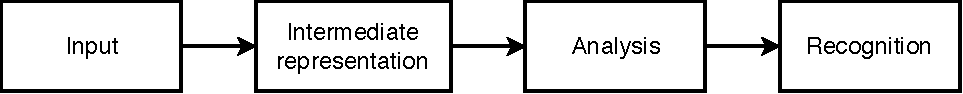
\includegraphics[scale=.9]{images/ddp}
	\label{fig:ddp_process}
	\caption{Quy trình kiểm tra sự tồn tại của mẫu thiết kế}
\end{figure}
Hầu hết những phương pháp kiểm tra sự tồn tại mã nguồn đề trải qua bốn giai đoạn, xác định kiểu dữ liệu đầu vào, xác định và xây dựng kiểu dữ liệu trung gian, tiến hành phân tích kiểu dữ liệu trung gian, áp dụng một số thuật toán hoặc không để đứa ra sự công nhận về sử tồn tại hay không của mẫu thiết kế trong mã nguồn.

\section{Bộ công cụ JCIA-VT}
JCIA-VT \cite{jcia-vt} là bộ công cụ phân tích và đảm bảo chất lượng mã nguồn cho các dự án J2EE sử dụng các framework Hibernate, Struts, Spring. Cụ thể, JCIA-VT áp dụng phân tích mã nguồn tĩnh để xây dựng một cấu trúc dữ liệu gọi là đồ thị phụ thuộc (Java Dependency Graph - JDG) nhằm thể hiện sự phụ thuộc giữa các thành phần trong mã nguồn dự án J2EE, sau đó sử dụng JDG để dự đoán thành phần của mã nguồn bị ảnh hưởng trong sự thay đổi của một tập hợp các thành phần mã nguồn. Ngoài ra, công cụ còn cung cấp các tính năng về phân tích luồng dữ liệu, phân tích cấu trúc cơ sở dữ liệu, phân tích độ phức tạp của dự án J2EE.

\noindent Hiện tại JCIA-VT triển khai dưới dạng ứng dụng Web trên nền trang Java Spring và JavaServer Faces. Công cụ này sẽ tiếp tục được bảo trì và phát triển thêm những tính năng nhằm tạo nên bộ công cụ hoàn chỉnh phụ vụ cho công tác phân tích và đảm bảo chất lương mã nguồn.
\section{Công cụ phân tích Java}
Công cụ phân tích Java (Java Parser - JP) \footnote{https://javaparser.org/} là bộ công cụ mã nguồn mở được chứng nhận bởi JetBrains \footnote{https://www.jetbrains.com/}. JP cung cấp các plug-in hỗ trợ \textit{parse}, \textit{analyze}, \textit{transform}, \textit{generate }đối với mã nguồn Java. Đồng thời JP cũng cung cấp các API, đo vậy ta hoàn toàn có thể sử dụng JP để hỗ trợ phát triển những công cụ khác. 
\subsection{Sử dụng JP để hỗ trợ phân tích mã nguồn Java}
JP là thành phần được sử dụng để hỗ trợ trong quá trình tiền xử lý mã nguồn. Sử dụng JP để phân tích mã nguồn, ta sẽ nhận được đầu ra là cây cú pháp trừu tượng (Abstract Syntax Tree - AST) tương ứng.
\begin{lstlisting}[language=Java,
caption={Sử dụng API của JS Core để tạo cây cú pháp trúc trừu tượng},label={code:jdt-ast-gen}]
CompilationUnit compilationUnit = StaticJavaParser.parse("class A { }");
Optional<ClassOrInterfaceDeclaration> classA = compilationUnit.getClassByName("A");
}
\end{lstlisting}
Hơn thế nữa, JP cũng cung cấp các API để ta thực hiện truy vấn tới những thành phần của một lớp trên cây cấu trúc
\begin{itemize}
	\item \texttt{public void visit(FieldDeclaration n, Void arg)}: Duyệt tới thuộc tính của một lớp.
	\item \texttt{public void visit(MethodDeclaration n, Void arg)}: Duyệt tới từng phương thức của một lớp, tại đây những đối tượng thể hiện cho phương cũng cung cấp các API để truy cập tới thành phần nhỏ hơn trong phương thức như tên phương thức, kiểu trả về, v.v.
	\item \texttt{public void visit(ClassOrInterfaceDeclaration n, Void arg)}: Duyệt tới một lớp, đồng thời đối tượng đại diện cho lớp sẽ cung cấp các phương thức truy cập tới kiểu lớp, tên, tính đóng gói.
\end{itemize}
\chapter{Phương pháp kiểm tra sự tuân thủ mẫu thiết kế cho dự án sử dụng Java}\noindent Mẫu thiết kế là tập hợp các luật nhằm mô tả cách giải quyết một vấn đề trong thiết kế có thể là vấn đề lặp lại nhiều lần trong dự án, là một khía cạnh của việc đảm bảo chất lượng mã nguồn, với những dự án công nghệ thông tin nói chung và dự án Java nói riêng. Ở các mẫu thiết kế hướng đối tượng, tập hợp các luật về thiết kế đem lại sự tương tác chặt chẽ giữa các thành phần trong mã nguồn với nhau. Những tương tác này có thể tổng quát hóa thành những dạng phụ thuộc nhất định. Đưa ra góc nhìn của mã nguồn về mặt cấu trúc. Do đó, phương pháp phát hiện sự tuân thủ mẫu thiết kế bên trong mã nguồn mà khóa luận này đễ xuất, đi theo hướng phân tích cấu trúc của mã nguồn.\\
\section{Tổng quan phương pháp}
Phương pháp phân tích cấu trúc sẽ dựa trên phấn tích tĩnh mã nguồn, việc phân tích mã nguồn tĩnh đem lại độ chính xác tốt và quá trình phân tích không bắt buộc mã nguồn có thể thực thi được. Đem lại sự linh hoạt cho phương pháp này, dữ liệu đầu vào có thể là toàn bộ mã nguồn hoặc bất cứ một hay nhiều thành phần của mã nguồn.\\\\
Hình \ref{fig:general_architecture} mô tả phương pháp kiểm tra sự tuân thủ mẫu thiết kế. Đầu tiên, dữ liệu đầu vào được tiền xử lý thành cây cấu trúc, thông qua cây cấu trúc tiến hành phân tích phụ thuộc bên trong mã nguồn, xây dựng đồ thị phụ thuộc. Quá trình này được thực hiện với cả mã nguồn dự án và mã nguồn của những mấu thiết kế được qui định, từ đó tìm ra sự tương đồng của mẫu thiết kế bên trong mã nguồn dự án. Nhằm kiểm tra được sự tuân thủ về mẫu thiết kế bên trong mã nguồn.
\begin{figure}[h]
	\centering
	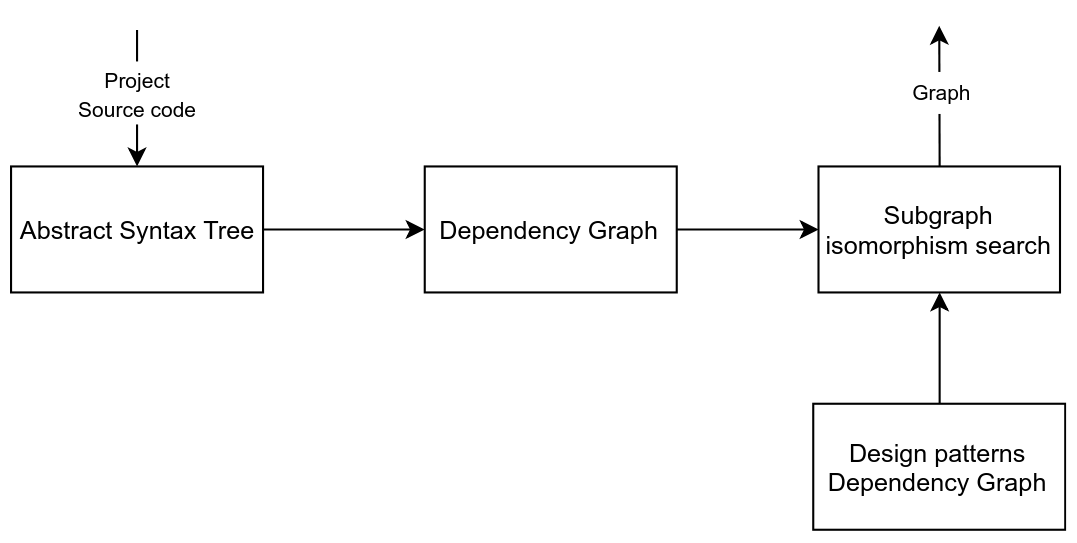
\includegraphics[scale=1.1]{images/general_architecture_3_1}
	\caption{Quá trình kiểm tra sự tuân thủ mẫu thiết kế của mã nguồn}
	\label{fig:general_architecture}
\end{figure}
\section{Tiền xử lý mã nguồn Java}
\subsection{Xây dựng cây cấu trúc}
Đối với phương pháp kiểm tra sự tuân thủ mẫu thiết kế mà khóa luận này đề xuất. Việc trực tiếp phân tích mã nguồn đầu vào là một giải pháp không tối ưu do sự phức tạp của mã nguồn, các thành phần không được sử dụng tới của mã nguồn ví dụ như các tệp tin xml, yml, v.v. Do đó, cần có một kiểu dữ liệu tường minh và thể hiện được toàn bộ thông tin, cấu trúc của mã nguồn. Nếu dùng trực tiếp mã nguồn sẽ gây khó khăn trong quá trình giải quyết bài toán và ảnh hưởng tới hiệu năng của công cụ được xây dựng. Vấn đề đặt ra, đó là mã nguồn cần được tiền xử lý, loại bỏ những thành phần không sử dụng, ánh xạ mã nguồn sang kiểu cấu trúc dữ liệu phù hợp. Cây cấu trúc được để xuất như là một kiểu cấu trúc dữ liệu phù hợp nhất thể hiện được toàn bộ cấu trúc của mã nguồn dự án với những ưu điểm như kiểu cấu trúc dữ liệu tượng minh, việc quan lý các đối tượng là dễ dàng nhằm mục đích phụ vụ cho việc phân tích cây cấu trúc sau này, hỗ trợ thể hiện phụ thuộc giữa các đối tượng bằng việc xây dựng liên kết giữa các nút trên cây.

\noindent \textbf{Định nghĩa: }(\textit{Cây cấu trúc} \cite{jcia}) Là một đồ thị liên thông với $T = (N,E)$ trong đó $N = \{n_1,n_2,n_3...n_n \}$ là tập các nút trên cây đại diện cho tệp, lớp, phương thức, biến, v.v. $E = \{(e_i,e_j) | e_i, e_j \in N \}$ mỗi cặp $e_ie_j$ là cặp hai nút cha con của cây.\\\\
Cây cấu trúc được xây dựng từ mã nguồn của dự án bằng cách ánh xạ lại những thông tin từ mã nguồn thành các nút trên cây. Hình \ref{fig:universe} mô tả cây cấu trúc từ mã nguồn dự án. Trong đó toàn bộ mã nguồn có cấu trúc là một thư mục gồm các tệp tin và thư mục con được đưa về dạng cây cấu trúc với các nút trên cây được ánh xạ về bốn loại: tệp tin (\textit{Java}), lớp, phương thức và một loại nút thể hiện cho những định dạng còn lại. Mỗi loại nút của cây chứa những thuộc tính khác nhau và thông tin về nút cha, con của chúng.

\noindent Những thông tin trên mỗi nút được phân tích từ cây cú pháp trừu tượng(Abstract Syntax Tree - AST) được sinh ra từ mã nguồn. Ngoài ra, quá trình sinh cây AST từ mã nguồn dự án, là một bước trung gian của quá trình xây dựng cây cấu trúc, kiến thức về cây AST và công cụ JP đã được trình bày tại \textbf{Chương 2} của khóa luận.
\begin{figure}[!htbp]
	\centering
	\vspace{0.5cm}
	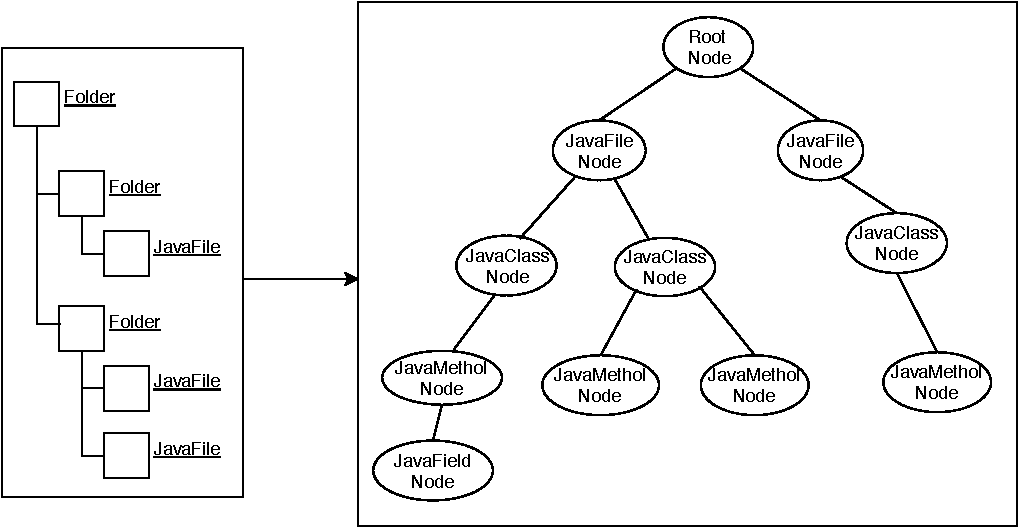
\includegraphics[scale=0.9]{images/structure_tree.pdf}
	\caption{Xây dựng cây cấu trúc từ mã nguồn}
	\label{fig:universe}
\end{figure}
\subsection{Xác định thuộc tính cho mỗi nút trên cây cấu trúc}
Xác định thuộc tính trên mỗi nút, nhằm ánh xạ đầy đủ thông tin cần thiết của mã nguồn lên cây cấu trúc mà ta cần xây dựng. Phục vụ quá trình phân tích phụ của mã nguồn. Quá trình xác định thuộc tính trên mỗi nút dựa trên việc phân tích mã nguồn ở các mức trừu tượng khác nhau như Class, Method, Variable, v.v.

\noindent Thành phần của một lớp gồm bốn phần chính: \textit{Class type, Class dependency, Class variables, Method }. Trong đó:
\vspace{-0.1cm}
\begin{itemize}
	\item \textit{Class type} của một nút (class) thể hiện nút đó đóng vai trò như một:\textit{ Class, Abstract class, Template class} hay \textit{Interface}.
	\item \textit{Class depedency} ở đây  ta xét tới phụ thuộc thừa kế của lớp, phụ thuộc thừa kế bao gồm hai loại: kế thừa từ một class, kế thừa từ Interface.
	\item \textit{Method} là định nghĩa một hành vi của lớp, \textit{Method} bao gồm các thành phần: \textit{Local variable, Return type, Input paramater}.
	\item  \textit{Class variables} là biến của một lớp được khởi tạo bên ngoài các \textit{Method}. \textit{Local variable} là biến chỉ được khai báo và sử dụng trong phạm vi \textit{Method}.  
	\item \textit{Return type} là kiểu dữ liệu mà phương thức sẽ trả về nếu \textit{Return type} là kiểu \textit{void} thì phương thức sẽ không trả về giá trị.
	\item \textit{Input paramter} xác định kiểu giá trị đầu vào cho phương thức.
\end{itemize}
Để rõ ràng hơn về quá trình xác định thuộc tính cho các nút của cây cấu trúc, ta tiến hành xem xét các ví dụ.
Hình \ref{fig:dependecy_extend} mô tả hai loại phụ thuộc kế thừa qua phương thức extends và inplements. Trong đó A là một Class thừa kế từ B là một Interface qua phương thức extend, C là một class thừa kế D qua phương thức implement với D là một abstract class.\\\\
\begin{figure}[!htbp]
	\centering
	\vspace{-1cm}
	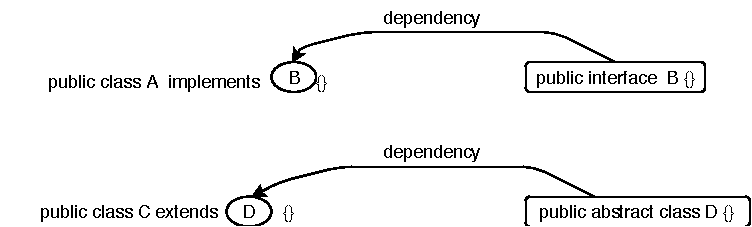
\includegraphics[scale=1.2]{images/class_dependency.pdf}
	\caption{Phụ thuộc thừa kế của lớp}
	\label{fig:dependecy_extend}
\end{figure}
\\
Hình \ref{fig:class_structure} Các thành phần cơ bản của \textit{Class}. Trong đó E là một Class với Access modifer là public, Class variable là sum với kiểu giá trị int và Access modifier là private, Method add() có kiểu trả về là int và hai biến đầu vào là a và b.\\
\begin{figure}[!htbp]
	\centering
	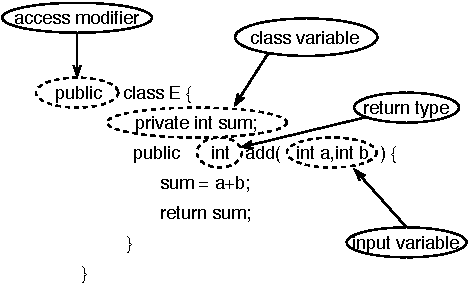
\includegraphics[scale=1.2]{images/class_method_structure.pdf}
	\caption{Các thành phần cơ bản trong class}
	\label{fig:class_structure}
\end{figure}
\newpage
\noindent Bảng 3.1 mô tả đầy đủ những thông tin cần xác định cho mỗi loại nút trên cây cấu trúc, nhằm phục vụ cho việc phân tích cấu trúc mã nguồn và xây dựng đồ thị phụ thuộc sẽ được trình bài tại mục \textbf{3.2} và \textbf{3.3} của chương này.
\begin{table}[!htbp]
	\centering
	\renewcommand{\arraystretch}{0.8}
	\begin{tabular}{|l|l|}
		\hline
		\textbf{Node} & \textbf{Popertiesoperties}                                        \\ \hline
		Class            & \begin{tabular}[c]{@{}l@{}}NameType\\ Access modifier\\ Extended Class\\ Implemented Class\\ Childrent Node: Field, Method\end{tabular} \\                                       \hline
		Method              & \begin{tabular}[c]{@{}l@{}}Name\\ NameReturn Type\\ Access modifier\\ Parameter\\ Body\end{tabular} \\ \hline
		Field               &\begin{tabular}[c]{@{}l@{}}Name\\ Value type\\ Access modifier\end{tabular} \\ \hline
	\end{tabular}
	\caption{Thuộc tính trên mỗi nút}
	\label{tbl:node_properties}
\end{table}

\noindent Việc trích xuất các thông tin từ mã nguồn cho các nút trên cây, được thực hiện thông qua AST. Với mỗi thành phần mã nguồn, ta sử dụng JP để sinh AST tương ứng với thành phần đó từ đó trích xuất các thuộc tính cần thiết cho mỗi nút trên cây cấu trúc.
Hình 3.5 mô tả một AST với một Class Java tương ứng. Trong đó một lớp Java được phân tách thành dạng cây với các nút gốc chứa các toán tử, các nút lá chứa các toán hạng. Ví dụ như return = 42, trong đó return là một toán tử ứng với `ReturnStatement' và `42' là toán hạng ứng với nút lá.
\begin{figure}[!htbp]
	\centering
	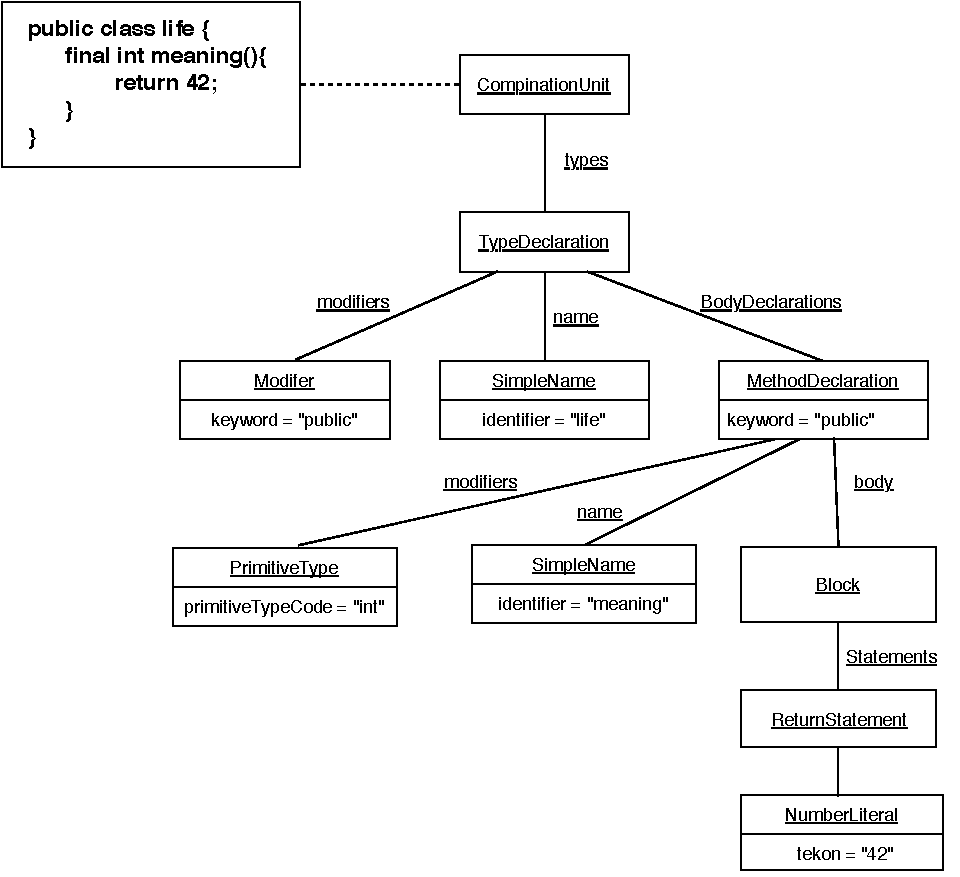
\includegraphics[scale=1]{images/ast_pdf}
	\caption{Abstract Syntax Tree đối với Java class}
	\label{fig:ast_for_java_class}
\end{figure}
\newpage
\section{Phân tích cấu trúc mã nguồn Java}
\indent Cấy cấu trúc thể hiện thể hiện chi tiết về cấu trúc của mã nguồn bao gồm các khía cạnh về tính hướng đối tượng bên trong mã nguồn. Phân tích cấu trúc mã nguồn nhằm xác định được những đặc điểm về mặt phụ thuộc giữa các thành phần mã nguồn được hình thành bới việc áp dụng những mẫu thiết kế bên trong mã nguồn. Xác định được những được những đặc nêu trên là tiền để để kiểm tra sự tuân thủ mẫu thiết kế bên trong mã nguồn.
\subsection{Phân tích phụ thuộc giữa các thành phần trong mã nguồn}
Đối với phương pháp mà khóa luận này đề xuất, việc phân tích phụ thuộc giữa các thành phân bên trong mã nguồn xoay quanh việc phân tích phụ thuộc giữa các lớp trong mã nguồn. Đối với loại phụ thuộc giữa các lớp trong mã nguồn Java bao gồm: Direct \& Indirect dependency, Polymorphism dependency, Inheritance Dependency, Use Dependecy,Behavior Dependency. Chi tiết về đăc trưng và ví dụ minh họa của từng loại phụ thuộc được trình bày như sau.

\noindent \textbf{Polymorphism dependency}: Là loại phụ thuộc khi có sự thừa kết giữa các đối tượng với nhau, tạo ra tính chất đa hình, đa trạng thái của đối tượng (Java) như tính chất liên kết động, upcasting, downcasting,v.v. Ở đây ta xem xét hai trường hợp của lọai phụ thuộc này. Trường hợp thứ nhất khi một Class thừa kế một Interface bằng phương thức Implement. Ví dụ Class, A  thừa kế một interface B, Class A sẽ thừa kế những phương thức của Interface C, tức là tại Class A những phương thức được Interface C định nghĩa sẽ được triển khai. Ngoài ra tham chiếu của Interface B có thể trỏ tới đối tượng của Class A, trong trường hợp đó đối tượng tạo được trỏ tới bởi B chỉ có thể thực hiện những phương thức mà B đã định nghĩa, nhưng phương thúc khác của A sẽ bị làm mờ đi. Trường hợp thứ hai, phụ thuộc xảy ra khi một class thừa kế một class khác thông qua phương thức extends. Ví dụ, class C thừa thế class D, lúc này ta coi D như là Class cha, với C là class con, C sẽ thừa hưởng mọi thuộc tính và phương thức của  D, do đó C có thể ghi đè những phương thức của D, ngoài ra, tham chiếu của Class D có thể trỏ tới đối tượng của class C. Hình 3.6 và 3.7 mô tả ví dụ về hai trường hợp mà ta đã đề cập.
\begin{figure}[!htbp]
	\centering
	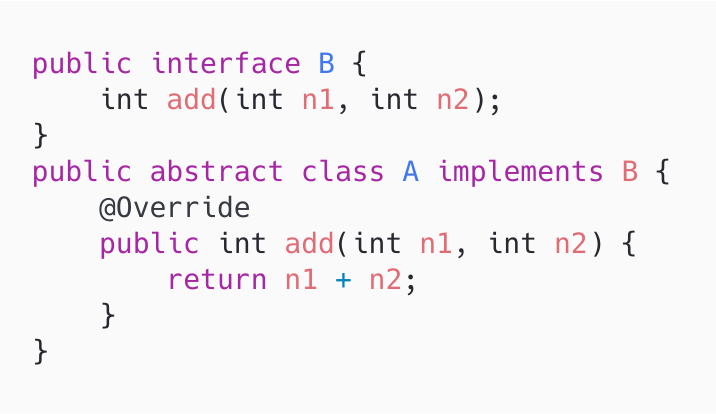
\includegraphics[scale=0.35]{images/AimplementsB}
	\caption{Mối quan hệ giữa một Class vớ một Interface qua phương thức Implements}
	\label{fig:A_implemets_B}
\end{figure}
\begin{figure}[!htbp]
	\centering
	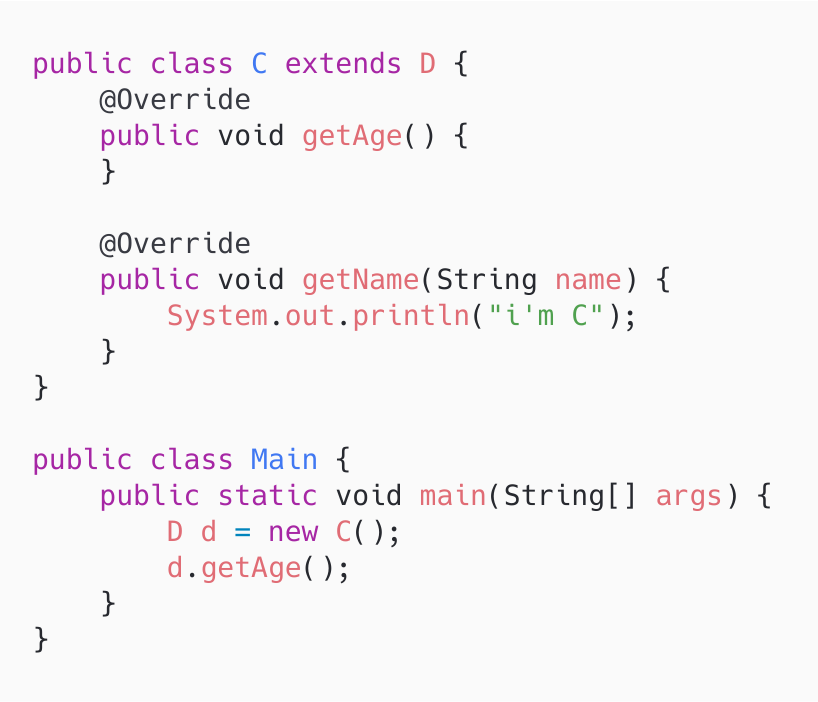
\includegraphics[scale=0.35]{images/CextendD}
	\caption{Mối quan hệ giữa một Class với một Class qua phương thức extends}
	\label{fig:CextendD}
\end{figure}
\newpage
\noindent \textbf{Inheritance Dependency}: Khi một Class có được các thuộc tính và phương thức của một Class khác. Những thuộc tính và phương thức này được quản lý theo thứ tự phân cấp từ lớp con tới lớp cha, việc xử lý phân cấp được quyết định trong quán trình chương trình đang thực thi bởi JVM. Ví dụ, ta có Class D thừa kế Class E với phương thức \textit{extends}, khi đó D sẽ thừa hưởng các phương thưc và thuộc tính của E. Trong trường hợp các phương thức và thuộc tính của D có \textit{Access modifier} là \textit{private}, khi đó đối tượng của Class A sẽ không thể gọi tới những thuộc tính, phương thức này. Hình \ref{fig:D_extends_E} mô tả mối quan hệ thừa kết giữa hai Class Java.\\\\
\begin{figure}[!htbp]
	\centering
	\vspace{-1.5cm}
	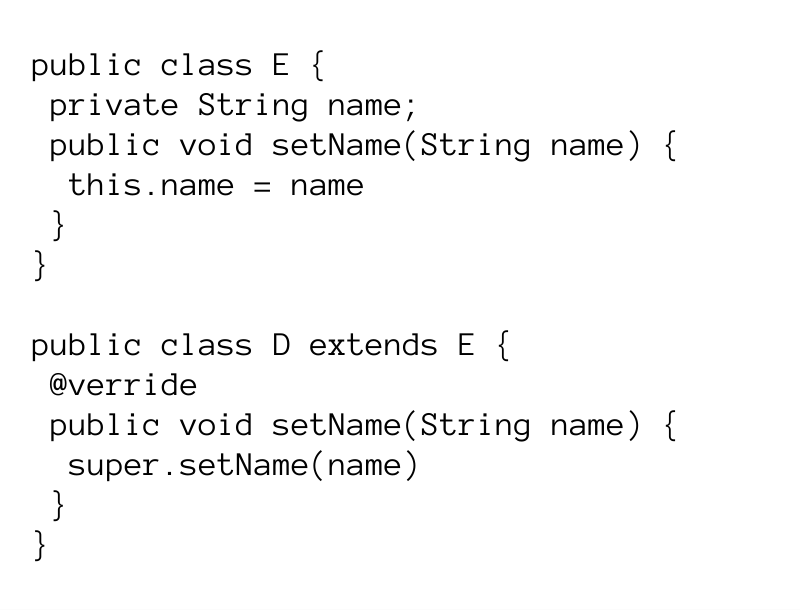
\includegraphics[scale=0.35]{images/D_extends_E}
	\caption{Mối quan hệ giữa một Class với một Interface qua phương thức Implements}
	\label{fig:D_extends_E}
\end{figure}\\
\textbf{Use Dependency}: Không giống với \textit{Inheritance Dependency} hay \textit{Polymorphism dependency}, Use Dependency thể hiện sự tương quan giữa các Class về mặt tương tác dữ liệu,khi các đối tượng của lớp này được sử dụng nhứ là thuộc tính, giá trị trả về, kiểu dữ liệu đầu vào, biến địa phương của phương thức của Class khác hoặc được sử dụng để khai kiểu cho một Generic Class.
\noindent Hình \ref{fig:use_dependency} mô tả \textit{Use dependency}. Chia làm hai ví dụ nhỏ. Ví dụ thứ nhất, đối tượng của Class A được khai báo là thuộc tính của Class B, những phương thức của Class B có kiểu trả về, kiểu dữ liệu đầu vào là đối tượng của Class A. Ví dụ thứ hai, Class C khai bảo kiểu Generic, và định nghĩa những phương thức sử dụng kiểu Generic, tức là kiểu dữ liệu mà Class định nghĩa cho các phương thức, thuộc tính của nó sẽ phụ thuộc vào kiểu dữ liệu được khai báo khi Class được sử dụng.
\begin{figure}[!htbp]
	\centering
	\vspace{-0.5cm}
	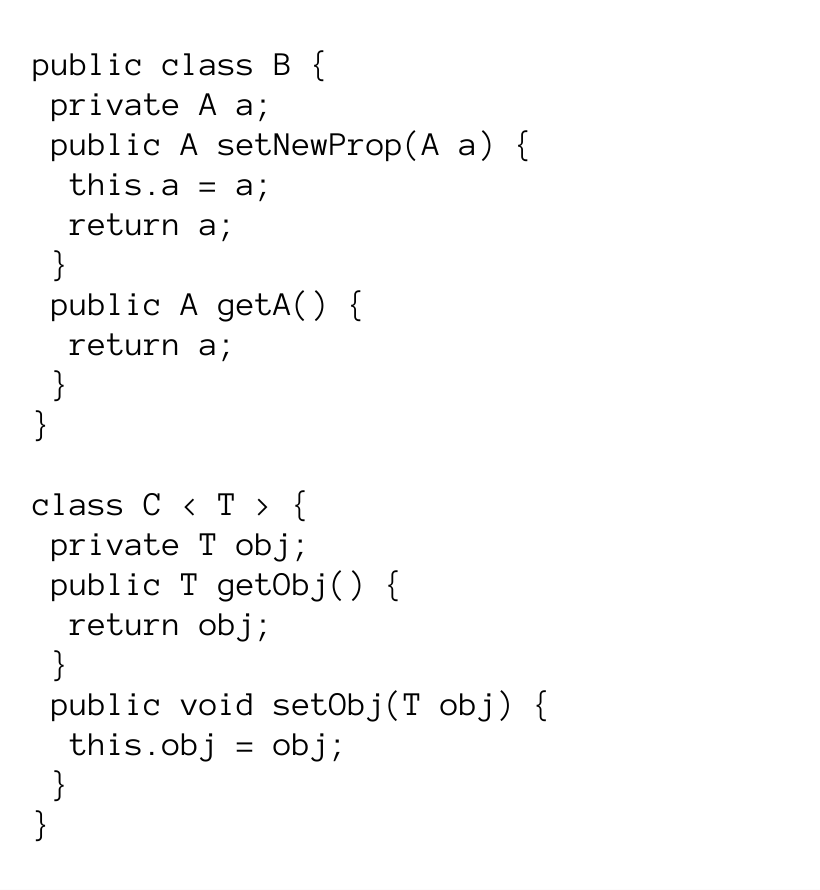
\includegraphics[scale=0.35]{images/use_dependency}
	\caption{Mô tả Use dependency}
	\label{fig:use_dependency}
\end{figure}
\\
\noindent \textbf{Behavior Dependency}: Phụ thuộc thể hiện hành vi của các dối tượng của mỗi Class, tức là sự tương tác của đối tượng của Class này với đối tượng của một Class khác. Điều kiện cần của loại phụ thuộc này đó là giữa Class có tồn tại Inheritance dependency.
\subsection{Xây dựng đồ thị phụ thuộc từ cây cấu trúc}
Đồ thị phụ thuộc nhằm thể hiện mối quan hệ về cấu trúc giữa các thành phần trong mã nguồn, sự tương tác giữa các thành phần như Class, Methol, Field, v.v. với nhau bên trong mã nguồn, tạo nên sự ảnh hưởng qua lại giữa chúng
việc phân tích và xây dựng đồ thị phụ thuộc xoay quanh phương pháp kiểm sự tuân thủ mẫu thiết kế bên trong mã nguồn dự án.
Đối với phương pháp mà khóa luận này đề xuất, đồ thị phụ thuộc được xây dựng là đồ thị có hướng.\\
\noindent \textbf{Đồ thị phụ thuộc} (\textit{Định nghĩa}): là một đồ thị có hướng $G = \{V,E \}$, trong đo $V = \{v_1,v_2,v_3..v_k\}$ là tập các đỉnh của đồ thị với mỗi đỉnh tương ứng với một Class trong mã nguồn, $E = \{ e_ie_j | e_i \in V, e_j \in V  \}$ là tập các cạnh đinh hướng của đồ thị từ đỉnh $e_i$ tới $e_j$. Trên mỗi cạnh nối hai đỉnh chứa thuộc tính thể hiện sự phụ thuộc giữa hai đỉnh (class) của đồ thị (mã nguồn).

\noindent Từ việc phân tích các loại phụ thuộc phái trên, ta tiến hành định nghĩa một tập những phụ thuộc, được hiểu như là các cạnh của đồ thị phụ thuộc. Tập các đỉnh là những Class. Được kiệt kê tất cả trong Bảng 3.2 và Bảng 3.3 \cite{orucc2016}
\begin{table}[!htbp]
	\centering
	\caption{Các loại đỉnh của đồ thị phụ thuộc}
	\label{tbl:java-class-type}
	\renewcommand{\arraystretch}{0.7}
	\begin{tabular}{|p{2.7cm}|p{8.7cm}|}
		\hline
		\textbf{Kí hiệu} & \textbf{Loại} \\ \hline
		C				& Class\\ \hline
		I				& Interface \\ \hline
		A				& Abstract class \\ \hline
		T				& Template class \\ \hline         
	\end{tabular}
\end{table}

\begin{table}[!htbp]
	\centering
	\caption{Các loại phụ thuộc Java}
	\label{tbl:field-ct}
	\renewcommand{\arraystretch}{0.9}
	\begin{tabular}{|l|l|}
		\hline
		\textbf{Kí hiệu} & \textbf{Ý nghĩa}                                        \\ \hline
		X               & class A extends class B                                        \\ \hline
		I               & class A implement class B                                                 \\
		\hline
		C               & class A create object of class B                                                \\
		\hline
		R              &  class A has the return type of class B             \\ \hline
		MC              & class A call a method of class B                          \\ \hline
		F              &  class A has the field type of class B   \\ \hline
		MR              &class A has a method with return type of class     \\ \hline
		MI              & \begin{tabular}[c]{@{}l@{}}class A has a method that has an input parameter\\ with the type of Class B \end{tabular} \\ \hline
		ML               & \begin{tabular}[c]{@{}l@{}}class A has a method that defines a local variable\\ with the type of class B\end{tabular} \\ \hline
		G              & class A uses class B in a generic type declaration   \\ \hline
		M               & class A has related with its method of class B \\ \hline
		O                &  class A overrides of class B \\  \hline
	\end{tabular}
\end{table}
\newpage
\noindent Để xây dựng đồ thị phụ thuộc ta duyệt lần lượt từng cặp nút (class) trên cây cấu trúc, với mỗi cặp nút ta tiến hành phân tích thông tin của mỗi nút nhằm kiểm tra sự tồn tại phụ thuộc giữa chúng. Nếu phụ thuộc tồn tại một đối tượng \textit{Dependency} được khởi tạo nhằm định danh phụ thuộc giữa hai nút.
\begin{thuattoan}[!htbp]
		\label{algo:dependency-analyze}
		\caption{$JavaDependencyAnalyze(Root)$}
		\SetKwInOut{Input}{Input}
		\SetKwInOut{Output}{Output}
		\Input{T là tập các nút trên cây cấu trúc}
		\Output{Graph là đồ thị phụ thuộc}
		$C$ = tập các nút lớp (Class Node) trên cây T \;
		$G$ = $New Grpah()$\;
		\ForEach{$c_i \in C$ , $C$ }{
			$d$ , $c_j$ = $analyzerClassLevel$($c_i$,$C$,$G$)\;
			
			\If{$d$ $not$ $empty$}{
					$new$ $Dependency$($c$,$c_j$,$d$)\;
			}
		
			
			$analyzerMethodLevel$($c_i$,$C$,$G$)\;
			\If{$d$ $not$ $empty$}{
				$new$ $Dependency$($c$,$c_j$,$d$)\;
			}
			
			$analyzerdFieldLevel$($c_i$,$C$,$G$)\;
			\If{$d$ $not$ $empty$}{
				$new$ $Dependency$($c$,$c_j$,$d$)\;
			}
		}
	
		\Return $G$\;
\end{thuattoan}
\subsection{Ví dụ minh họa}
\noindent Để hiểu rõ hơn về đồ thị phụ thuộc ta xem xét ví dụ Hình \ref{fig:example_graph_dependency}. Là độ thị phụ thuộc sinh ra từ một đoạn mã nguồn. Trong đó, đỉnh của đồ thị diểuiểu thị cho các lớp , \textbf{C} tương ứng với class và \textbf{I} tương ứng với Interface. Những class, interface này tương tác lẫn nhau qua những phụ thuộc như \textbf{MI} \textit{: class A has a method that has an input parameter with the type of Class B}, \textbf{ML} : \textit{class A has a method that defines a local variable with the type of class B}, v.v.\\
\begin{figure}[!htbp]
	\centering
	\vspace{-1cm}
	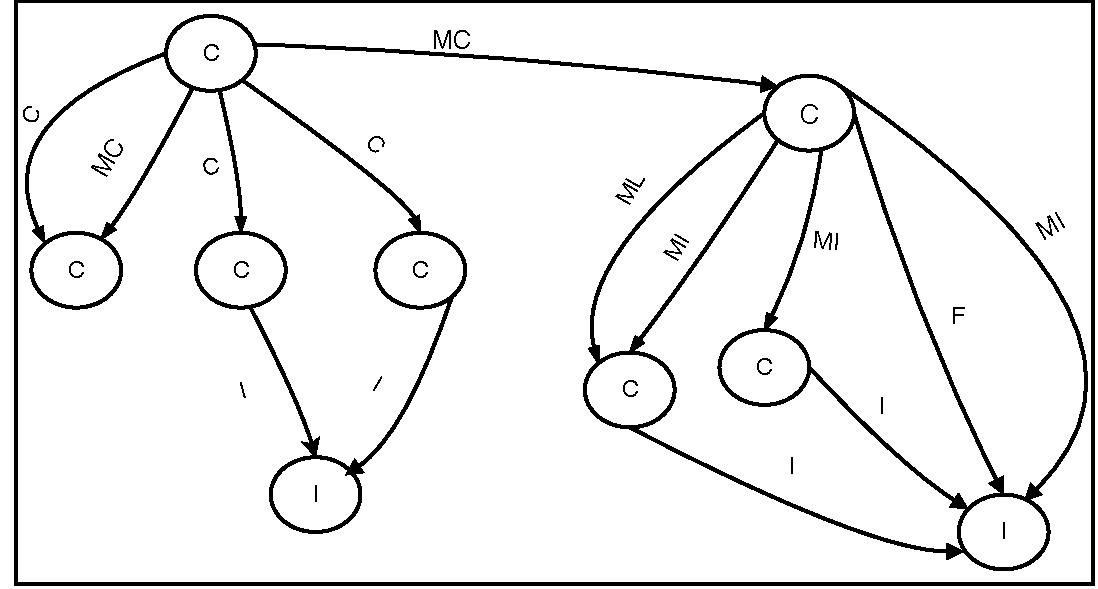
\includegraphics[scale=1]{images/dependency_graph}
	\caption{Ví dụ minh họa về đồ thị phụ thuộc}
	\label{fig:example_graph_dependency}
\end{figure}\\
Đồ thị này là tiền đề đê kiểm tra sự tuân thủ mẫu thiết kế trong mã nguồn sẽ được trình bày ở phần sau.
\pagebreak
\section{Kiểm tra sự tuân thủ mẫu thiết kế bên trong mã nguồn}
Quá trình kiểm tra sự tuân thủ mẫu thiết kế trong mã nguồn, tức là kiểm tra sự tồn tại của một mẫu thiết kế bên trong mã nguồn. Đầu vào của phần này gồm hai thành phần. Thứ nhất, \textbf{đồ thị phụ thuộc} của mã nguồn dự án. Thứ hai, \textbf{đồ thị phụ thuộc} của những mẫu thiết kế. Ta sẽ đi tiến hành kiểm tra sự tồn tại của từng mẫu thiết kế bên trong mã nguồn. 
Đầu vào của bài toán sẽ là hai đồ thị có hướng. Bản chất của vấn đề sẽ là tìm kiếm sự tồn tại của một đồ thị bên trong một đồ thị khác. Đo đó, thuật toán tìm kiếm đồ thị đẳng cấu \textbf{VF2 algorithm for the Subgraph Isomorphism Problem} được đề xuất để giái quyết bài toán.


\noindent \textbf{Ý tưởng của giải thuật VF2} \cite{vf2}:
\begin{itemize}
	%\item Assume the problem is to find a subgraph in G1 isomorphic to the graph G2.
	\item Ta cần tím kiếm một đồ thị con của đồ thị G1 mà đẳng cấu với đồ thị G2.
	%\item The main idea is to construct a state S which contains a correct partial match between nodes of G1 and G2
	\item  Ý tương ở đây là đi xây dựng một trạng thái S chứa một phần các đỉnh của G1 và G2.
	%\item M(s) identifies two sub graphs of G1 and G2, say G1(s) and G2(s), obtained by selecting from G1 and G2 only the nodes included in M(s),and the branches connecting them. Where s is a state of the matching process. 
	
	\item M(s) là tập ánh xạ xác định hai đồ thị con của G1 và G2, gỉa sử là G1(s) và G2(s) thu được bằng cách chọn từ G1 và G2 cách cặp đỉnh chỉ chứa trong M(s) và các cạnh kết nối giữa chúng. Trong đó s là trạng thái của quá trình khớp đồ thị
	%\item The main problem is extending M(s) with new branches.
	\item Ta cần mở rộng tập M(s) với những cặp đỉnh mới.
	%\item An extension of S is adding a pair (n,m) where n belongs to G1 and m belongs to G2.
	\item Với mỗi trạng thái s, ta tính toán những cặp ánh xạ (n,m) là ứng viên cho  M(s)
	%\item Feasibility rules is a set of rules that are able to verify the consistency conditions, making possible the generation of consistent states only.
	\item Tập các luật được định nghĩa trước nhằm xác định một cặp đỉnh có là ánh xạ đúng hay không. Xác định cặp ánh xạ (n,m) có phải là ảnh xạ chính xác hay không. Việc thêm một cặp (n,m) vào M(s), sẽ chuyển trạng thái của s tới s'.
\end{itemize}
\pagebreak
\subsection{Xây dựng đồ thị đầu vào cho giải thuật VF2}
Đồ thị đầu vào cho giải thuât là một đồ thị có hướng $G = (V,E)$. Trong đó V là các đỉnh tương ứng với các nút (class) trong cây cấu trúc, $E \subseteq V \times V$ là tập các cạnh với thuộc tính trên cạnh là phụ thuộc giữa các đỉnh trên đồ thị 

\noindent Để xây dựng đồ thị gọi cho giải thuật VF2, ta cần trích xuất các đỉnh (class) và các phụ thuộc giữa chúng từ cây cấu trúc. Các bước để xây dựng đồ thị được trình bày ở Thuật toán \ref{algo:get-input-for-jgraph}.

\begin{thuattoan}
	\label{algo:get-input-for-jgraph}
	\caption{Xây dựng đồ thị từ cây cấu trúc}
	\SetKwInOut{Input}{Input}
	\SetKwInOut{Output}{Output}
	\SetKwInOut{Use}{Use}
	\Input{$root$: nút gốc cây cấu trúc}
	\Output{$G = (V,E)$: đồ thị gọi}
	\Use{$getAllClassNode(root)$ các nút (class) của cây}
	\Use{$getDepedencies()$ phụ thuộc của một nút}
	N = $T.getAllClassNode(root)$\;
	G = $Graph()$\;
	 D = $Set()$\;
	\ForEach{$n \in $N}{
		D.$add(n.getDepedencies())$\;
	}
	G.$addNode($N$)$\;
	\ForEach{$d \in $D}{
		G.$addEdge(d)$\;
	}
	\Return G \;
	
\end{thuattoan}

\subsection{Kiếm tra sự tuân thủ mẫu thiết kế}
Như ý tưởng đã trình bày ở trên, việc kiểm tra sự tuân thủ mẫu thiết kế, trình là bài toán tìm kiếm đồ thị con-đẳng cấu giữa hai đồ thị phụ thuộc đại diện cho mã nguồn và mẫu thiết kế. Quá trình tìm kiếm đồ thị đẳng cấu là quá trình ánh xạ các cặp đỉnh từ hai đồ thị. Việc này tạo nên một không gian trạng thái của những đáp án đổi với mỗi trường hợp ánh xạ của mỗi cặp định khác nhau của hai đồ thị. Quá trình này được mô tả như Hình \ref{fig:vf2_example}.
\begin{figure}[!htbp]
	\centering
	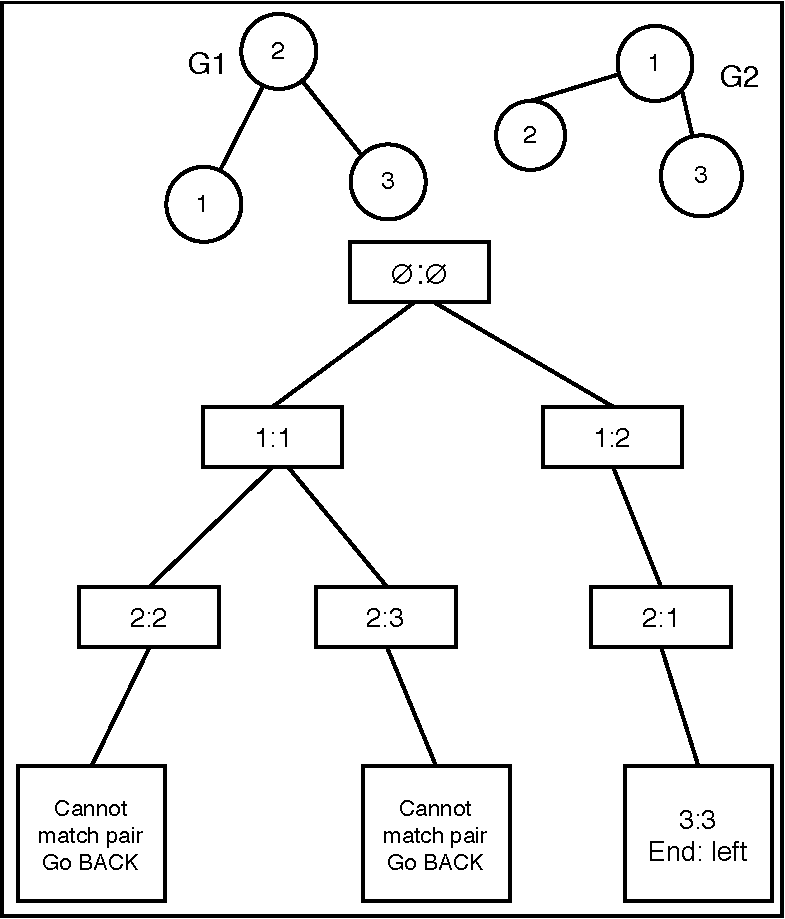
\includegraphics[scale=0.7]{images/_vf2_example.pdf}
	\caption{Mô tả thuật toán VF2}
	\label{fig:vf2_example}
\end{figure}\\
\noindent Giải thuật VF2 ra đời nhằm tối ưu quá trình tìm kiếm đáp án tối ưu trong không gian trạng thái, bằng phương pháp đề xuất tập các luật có thể xác định trạng thái tối ưu trong quá trình tìm kiếm cặp đỉnh ánh xạ giữa hai đồ thị, ngoài ra cũng làm giảm số lượng trạng thái được tạo ra trong quá trình tìm kiếm. Tập các luật được biểu diễn như sau:
\indent \indent \indent \indent \indent
\begin{equation}
	F(s,n,m) = F_{syn}(s,n,m) \wedge F_{sem}(s,n,m)
\end{equation}
Trong đó $F_{syn}$ là tập các luật đánh giá trạng thái dựa trên cấu trúc của đồ thị, $F_{sem}$ đánh giá trạng thái dựa trên các thuộc tính tại đỉnh, cạnh của đồ thị.
\noindent Tập các luật được định nghĩa cho giải thuật VF2 như sau \cite{vf2_1368}:
\begin{enumerate}
	\item Feasibility Rules 
	\begin{itemize}
		\item $F_{syn}(s,n,m) = R_{pred} \wedge R_{succ} \wedge R_{out} \wedge R_{new}$
		\item $R_{pred}(s,n,m) \iff\\ (\forall n \in M_1(s) \cup Pred(G_1,n)') \exists m' \in Pred(G_2,m) | (n',m') \in M(s)) \wedge\\
		(\forall m' \in M_2(s) \cup Pred(G_2,m) \exists n' \in Pred(G_1,n) | (n',m') \in M(s))$
		\item $R_{succ}(s,n,m) \iff\\ (\forall n \in M_1(s) \cup Succ(G_1,n)') \exists m' \in Succ(G_2,m) | (n',m') \in M(s)) \wedge\\ 
		(\forall m' \in M_2(s) \cup Succ(G_2,m) \exists n' \in Succ(G_1,n) | (n',m') \in M(s))$
		\item $R_{in}(s,n,m) \iff\\ (Card(Succ(G_1,n) \cup T^{in}_1(s)) \geq  Card(Succ(G_2,m) \cup T^{in}_2(s))) \wedge\\
		(Card(Pred(G_1,n)\cup T^{in}_1(s)) \geq Card(Pred(G_2,m)\cup T^{in}_2(s)))$ 
		\item $R_{out}(s,n,m) \iff\\ (Card(Succ(G_1,n) \cup T^{out}_1(s)) \geq  Card(Succ(G_2,m) \cup T^{out}_2(s))) \wedge\\
		(Card(Pred(G_1,n)\cup T^{out}_1(s)) \geq Card(Pred(G_2,m)\cup T^{out}_2(s)))$ 
		\item $R_{new}(s,n,m) \iff\\ Card(\tilde{N}_1(s) \cup Pred(G_1,n)) \geq Card(\tilde{N}_2(s) \cup Pred(G_2,n)) \wedge\\
		Card(\tilde{N}_1(s) \cup Succ(G_1,n)) \geq Card(\tilde{N}_2(s) \cup Succ(G_2,n))$
	\end{itemize}
	\item Semantic Feasibility
	\begin{itemize}
		\item $F_{s,n,m} \iff n \approx m  \wedge \forall(n',m') \in M(s),(n,n') \in B_1 \Rightarrow (n,n')\
		 \wedge \forall(n',m') \in M(s),(n',n) \in B_1 \Rightarrow (n',m) \approx (m',m)$
	\end{itemize} 
\end{enumerate}
\newpage
\noindent Các bược của giải thuật VF2 \cite{vf2_1368} sẽ được trình bày chi tiết ở Thuật toán \ref{algo:VF2}.
\begin{thuattoan}[!htbp]
	\label{algo:VF2}
	\caption{$VF2$}
	PROCEDURE Match(s)\\
	\SetKwInOut{Input}{Input}
	\SetKwInOut{Output}{Output}
	\hspace{5mm}\Input{an intermediate state $s$; the initial state $s_0$ has $M(s_0) = \emptyset $}
	\hspace{5mm}\Output{the mappings between the two graphs}
	\hspace{5mm}IF $M(s)$ covers all the node of G2\\
	\hspace{10mm} \Return M(s)
	
	\hspace{5mm}ELSE\\
	\hspace{10mm} Compute the set $P(s)$ of the paris candidate for inclusion in $M(s)$\\
	\hspace{10mm} FOREACH	$p \in P(s)$ \\
	\hspace{10mm} IF the feasibility reles successd for the inclusion of p in $M(s)$\\
	\hspace{20mm} Compute the state $s'$ obtained by adding p to $M(s)$\\
	\hspace{20mm} CALL Match($s'$)\\
	
	\hspace{15mm} END IF
	
	\hspace{10mm}END FOREACH\\
	\hspace{10mm}Restore data structures\\
	\hspace{5mm}END IF\\
	END PROCEDURE Match
\end{thuattoan}\\
Nếu mẫu thiết kế có tồn tại trong mã nguồn, kết quả trả về sẽ là một tập ánh xạ giưa toàn bộ đỉnh của đồ thị từ mẫu thiết kế với các đỉnh tưởng ứng trên đồ thị của mã nguồn.\\
Từ việc giải quyết được bài toán kiểm tra sự tuân thủ của mẫu thiết kế trong mã nguồn, chương tiếp theo khóa luận sẽ trình bày chi tiết cách triển khai phương pháp đã trình bày vào xây dựng công cụ trong thực tế.
\chapter{Công cụ và thực nghiệm}
Trong chương này, khóa luận sẽ trình bày về kiến trúc và cách cài đặt của công cụ cho phương pháp đã được trình bày ở chương 3 bao gồm, kiến trúc tổng quan của bộ công cụ JCIA-VT, kiến trúc của công cụ \textit{Kiểm tra sư tuân thủ mẫu thiết kế bên trong mã nguồn} mà khóa luận đề xuất và xây dựng và tích hợp với bộ công cụ với JCIA-VT. Thêm vào đó, đưa ra một số thực nghiệm để tiến hành phân tích thử nghiệm và đánh giá công cụ.

\newpage
\section{Kiến trúc và cài đặt công cụ}
\subsection{Tổng quan bộ công cụ JCIA-VT}
Ở phần này sẽ trình bày về kiến trúc của bộ công cụ JCIA-VT. Kiến trúc của JCIA-VT được mô tả trong Hình 4.1. JCIA-VT được xây dựng dưới dạng một ứng dụng Web dựa trên hai Framework Java là Spring và JavaServer Faces (JSF) bao gồm các mô-đun chính:

\noindent \textbf{Preprocessor}: Mô-đun này chịu trách nhiệm nhận dạng loại dữ liệu đầu vào, bao gồm các mô-đun nhỏ đảm nhận các chức năng như nhận dạng nền tảng, công nghệ mà dự án sử dụng, ví dụ như: Java Spring, Java Strust, C$\#$, v.v. Đầu vào là mã nguồn dự án dưới dạng tệp tin nén. Mã nguồn dự án sẽ được giải nén, dựa vào các mô-đun \textit{Language Detector}, \textit{Frameword Detector}, \textit{Configuration Detector} bằng các phân tích những tập tin cấu hình, tập tin mã nguồn để nhận dạng loại ngôn ngữ, công nghệ mà dự án sử dụng.

\noindent \textbf{Parser}: Mô-đun này nhận đầu vào là toàn bộ mã nguồn dự án. Mã nguồn sẽ được phân tích, mỗi mô-đun nhỏ phụ trách việc phân tích đối với từng loại mã nguồn khác nhau. Ngoài ra, cấu trúc dữ liệu được xây dựng cũng phụ thuộc vào từng loại công nghệ, mã nguồn là được tiến hành xây dựng. Ví dụ: đối với dự án sự dụng mã nguồn Java, cây cấu trúc sẽ được xây dựng.

\noindent \textbf{Dependency Analyzer}:Bao gồm nhiều mô-đun nhỏ phụ trách phân tích phụ thuộc cho từng loại ngôn ngữ, công nghệ. Đầu vào là mã nguồn đã được phân tích từ mô-đun \textit{Parser}, tùy vào mỗi công nghệ, ngôn ngữ mà dự án sử dụng mà mô-đun nào sẽ được gọi tới. Ví dụ: đối với dự án Java, mô-đun \textit{Java Dependency Analyzer} sẽ được gọi tới, tiến hành phân tích các phụ thuộc tồn tại bên trong mã nguồn trả về \textit{cây phụ thuộc}.

\noindent \textbf{Change Impact Analyzer}: Là mô-đun phân tích thay đổi cho mã nguồn, đầu vào là một tập thay đổi, đầu ta là tập mã nguồn sẽ bị ảnh hưởng. Đây là một trong những mô-đun đảm nhiệm chức năng chính cho JCIA-VT. Quá trình phân tích ảnh hưởng được thực hiện dựa trên giải thuật WAVE-CIA.

\noindent \textbf{Supporting Service Analyzer}: Ngoài chức năng \textit{Phân tích ảnh hưởng}, JCIA-VT còn cung cấp thêm nhiều tính năng, phục vụ cho quá trình kiểm thử hồi quy (Regession Testing Tools). Bao gồm các mô-đun cung cấp các tính năng như: phân tích luồng dữ liệu (Data Flow Diagram Analyzer), phát hiện sự tuân thủ mẫu thiết kế (Detect Design Pattern), phân tích độ phức tạp của mã nguồ ( Cyclomatic Analyzer) .v.v.\\
\textbf{Visualyzer}: Mô-đun thể hiện đầu ra của mã của những tính năng từ JCIA-VT 
\begin{figure}[h]
	\centering
	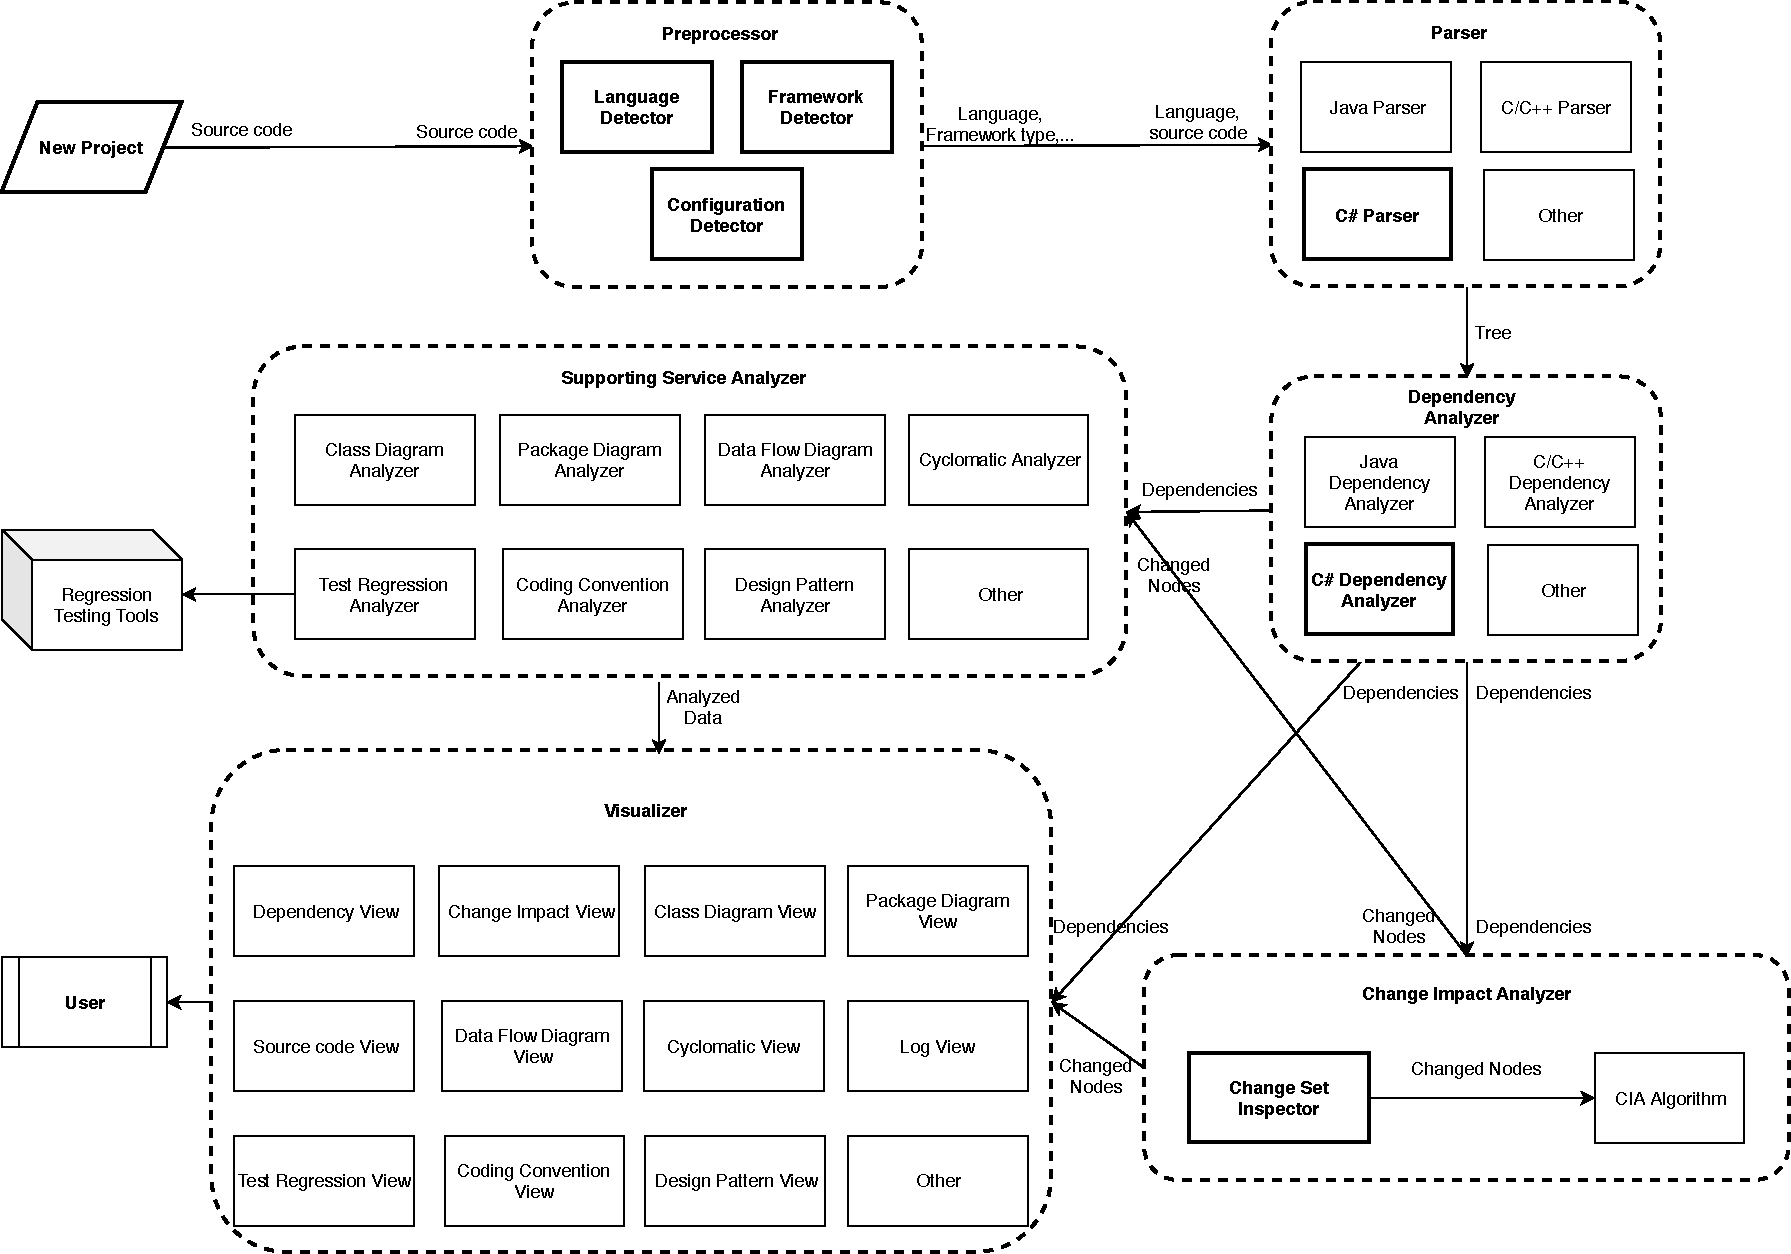
\includegraphics[scale=0.6]{images/architexture}
	\caption{Tổng quan kiến trúc JCIA-VT}
	\label{fig:architexture}
\end{figure}
\subsection{Kiến trúc và cài đặt công cụ kiểm tra sự tuân thủ mẫu thiết kế bên trong mã nguồn}
Phần này sẽ trình bày về kiến trúc chi tiết của mô-đun kiểm tra sự tuân thủ mã nguồn trong bộ công cụ JCIA-VT.

\noindent Mô-đun được tích hợp trực tiếp bên trong mã nguồn backend của bộ công cụ JCIA-VT. Kiến trúc chi tiết được mô tả như trong hình \ref{fig:detect_design_pattern_architexture}, kiến trúc này được thiết kế dựa trên phương pháp đã mô tả ở phần 3 của khóa luận. Bao gồm bốn thành phần chính:
\begin{figure}[!htbp]
	\centering
	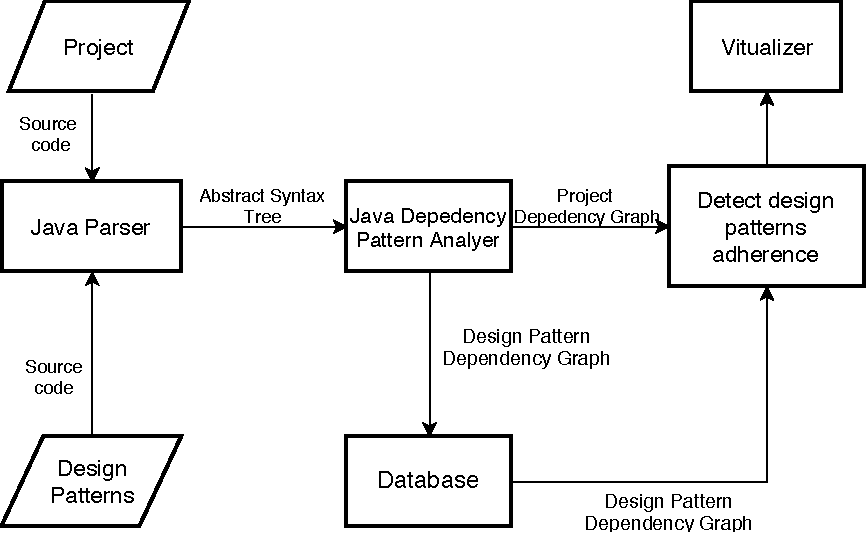
\includegraphics[scale=1]{images/c4_architexture.pdf}
	\caption{Kiến trúc }
	\label{fig:detect_design_pattern_architexture}
\end{figure}\\
Kiến trúc của công cụ bao gồm năm mô-đun chính bao gồm: xử lý dữ liệu đầu vào (preprocessor), phân tích mã nguồn (Java Design Pattern Analyzer), cơ sở dữ liệu (Database), phát hiện mẫu thiết kế (Detecting Design Pattern), mô hình hóa đầu ra (Visualizer). Do quá trình tích hợp với bộ công cụ JCIA-VT mô-đun tiền xử lý dữ liệu đầu vào sẽ được tái sử dụng, ngoài ra những mô-đun khác của công cụ sẽ cần được xây dựng mới và sẽ được tích hợp thành mội gói bên trong mã nguồn của bộ công cụ  JCIA-VT.

\begin{itemize}
	\item \noindent \textbf{Java Design Pattern Analyzer}: Là thành phần chịu trách nhiệm phân tích mã nguồn. Đầu vào là mã nguồn Java, đầu ra là đồ thị phụ thuộc của mã nguồn. Đầu tiên cây AST sẽ được sinh ra từ mã nguồn, tiếp đo quá trình xây dựng cây cấu trúc được thực hiện. Từ cây cấu trúc, việc phân tích phụ thuộc được tiến hành.
	%\begin{itemize}
	%	\item \textit{ddp.dom}: Định cấu trúc các nút trên cây cấu của mã nguồn
	%	\item \textit{ddp.parser}: Phân tích mã nguỗn, xây dựng cây cấu trúc từ mã nguồn
	%	\item \textit{ddp.analyzer}: Phân tích cây cấu trúc, thực hiện gắn phụ thuộc giữa các nút trên cây. Những phụ thuộc cần phân tích đã được định nghĩa tại chương 3 mục 3.3.
	%	\item \textit{ddp.graph}: Xây dựng đồ thị phụ thuộc, với đầu vào là cây cấu trúc của mã nguồn dự án.
	%\end{itemize}
	\item \noindent \textbf{Database}: Quản lý việc lưu trữ cây cấu trúc của mã nguồn cũng như những mẫu thiết kế đã được định nghĩa của dự án. Sự dụng hệ quản trị cơ sở dữ liệu H2. Phần này được xây dựng dựa trên gói \textit{core.DAO} của bộ công cụ JCIA-VT
	\item \noindent \textbf{Detecting Design Pattern}: Chịu trách nhiệm kiểm tra sự tồn tại của mẫu thiết kế bên trong mã nguồn. Sử dụng giải thuật VF2 như đã được trình bày tại chương 3 mục 3.4. Với đầu vào là cây cấu trúc của mã nguồn cùng với cây cấu trúc của mẫu thiết kế đã được định nghĩa.
	\item \noindent \textbf{Visualizer}: Cung cấp giao diện thể hiện kết quả của quá trình kiểm tra sự tồn tại của mẫu thiết kế bên trong mã nguồn. Kết quả thể hiện dưới dạng đồ thị được triển khai bằng Javascript dựa trên thư việc Visjs \footnote{http://visjs.org/}. Giao tiếp
\end{itemize}
\newpage
\section{Triển khai}
Hiện tại công cụ đã được phát triển và đặt, trên một phiên bản mới của JCIA-VT. Cung cấp những giao diện và tính năng mới liên quan tới việc kiểm tra sự tuân thủ của mẫu thiết kế bên trong mã nguồn.
\subsection{Giao diện tải nên mẫu thiết kế}
Sau khi đăng nhập thành công vào hệ thống, để có thể tiến hành phân tích, kiểm tra sự tuân thủ mẫu thiết kế bên trong mã nguồn. Người dùng cần tải lên những mẫu thiết kế đã được định nghĩa trước mà dự án sẽ được yêu cầu phát triển dựa trên những mẫu thiết kế đó. Mẫu thiết kế tải lên, nên chỉ tồn tại những tập tin Java và cần được đóng gói thành tập tin nén. Hình \ref{fig:ds_upload_example} mô tả màn hình tải nên một mẫu thiết kế mới.
\begin{figure}[!htbp]
	\centering
	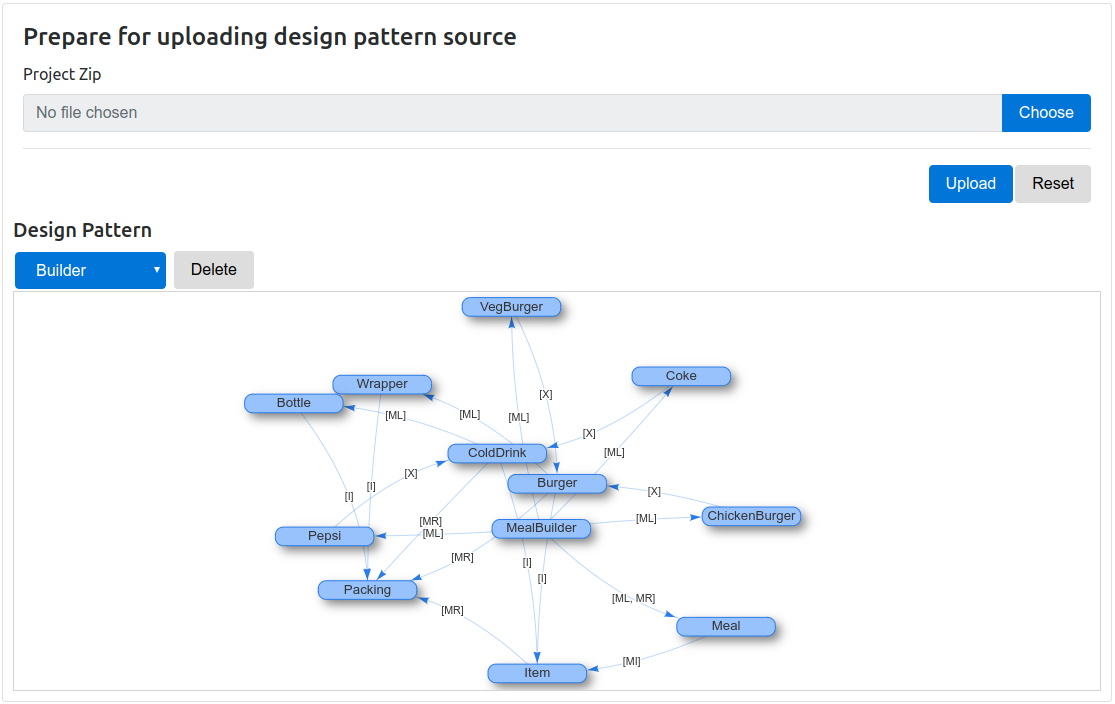
\includegraphics[scale=0.36]{images/ds_upload_example}
	\caption{Giao diện tải lên mẫu thiết kế}
	\label{fig:ds_upload_example}
\end{figure}\\
Giao diện tải lên mẫu thiết kế cung cấp hai tính năng chính. Thứ nhất, tải lên và quản lý mẫu thiết kế. Khi người dùng tải lên mẫu thiết kế mới, mã nguồn của mẫu thiết kế sẽ được tiến hành xử lý để xây dựng đồ thị phụ thuộc thể hiện cấu trúc của mã nguồn sau đó được lưu trữ trên cơ sở dữ liệu nhằm phục vụ công việc kiểm tra sự tuân thủ mẫu thiết kế. Thứ hai: quản lý và hiển thị đồn thị phụ thuộc của mẫu thiết kế, người dùng có thể thêm hoặc xóa mẫu thiết kế, đồng thời giao diện cũng cung cấp cửa sổ hiển thị đồ thị phụ thuộc của mẫu thiết kế.
\subsection{Giao diện phát hiện mẫu thiết kế bên trong mã nguồn}
Sau khi tiến hành tải lên những mẫu thiết kế được yêu cầu trong việc phát triển mã nguồn. Ta tiến hành phân tích mã nguồn để kiểm tra sự tuân thủ của mã nguồn đối với những mẫu thiết kế đã được qui định. Ở phân này, ta sẽ trình bày lần lượt từng bươc một theo luồng điều khiển, bao gồm quá trình tải liên mã nguồn dự án, quá trình phân tích ảnh hưởng và quá trình kiểm tra sự tuân thủ mã mẫu thiế kế bên trong mã nguồn của dự án.
Đầu tiên, mã nguồn sẽ được tiến hành tải nên, tại giao diện tại lên mã nguồn dự án như Hình \ref{fig:upload_project_source_code}. Cần thêm được dẫn tới thư mục chứa mã nguồn như trong giao diện mô tả.
\begin{figure}[h]
	\centering
	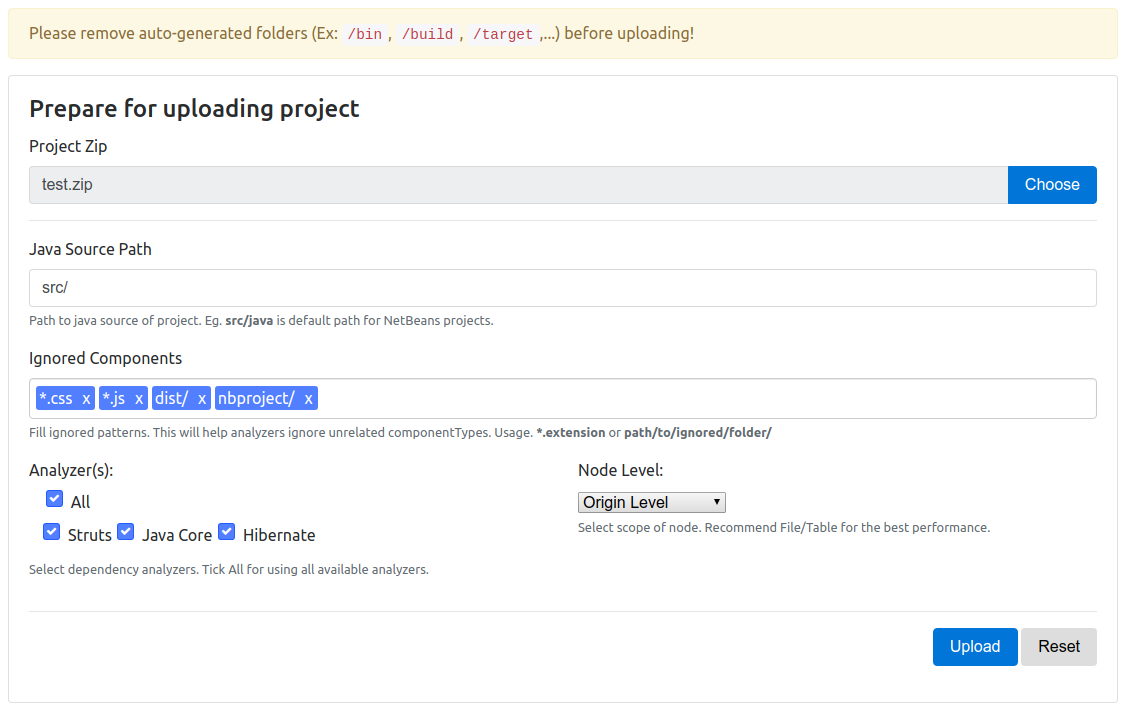
\includegraphics[scale=0.35]{images/upload_project}
	\caption{Giao diện tải lên mã nguồn dự án}
	\label{fig:upload_project_source_code}
\end{figure}\\
Sau khi nhấn chọn \textit{Upload}, hệ thống chuyển tới giao diện lịch sử và đồng thời tiến hành phân tích mã nguồn dự án. Giao diện lịch sử sẽ được thể hiện như trong Hình \ref{fig:history_screen}. Bao gồm thông tin về quá trình phân tích mã nguồn, thông tin về mã nguồn của các dự án khác nhau.
\begin{figure}[h]
	\centering
	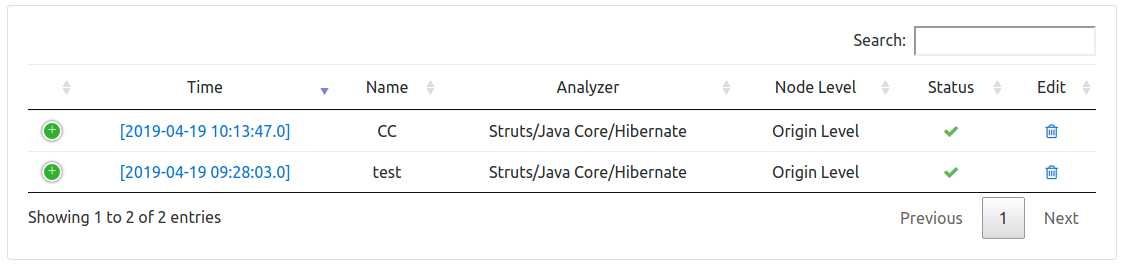
\includegraphics[scale=0.38]{images/history_screen}
	\caption{Giao diện màn hình lịch sử}
	\label{fig:history_screen}
\end{figure}\\
Quá trình phân tích mã nguồn hoàn thành, giao diện làm việc chính của JCIA-VT sẽ hiển thị khi người dùng chọn một trong các dự án tại danh sách được hiển thị như trên hình \ref{fig:history_screen}. Giao diện làm việc chính của JCIA-VT bao gồm nhiều màn hình khác nhau.
\begin{figure}[h]
	\centering
	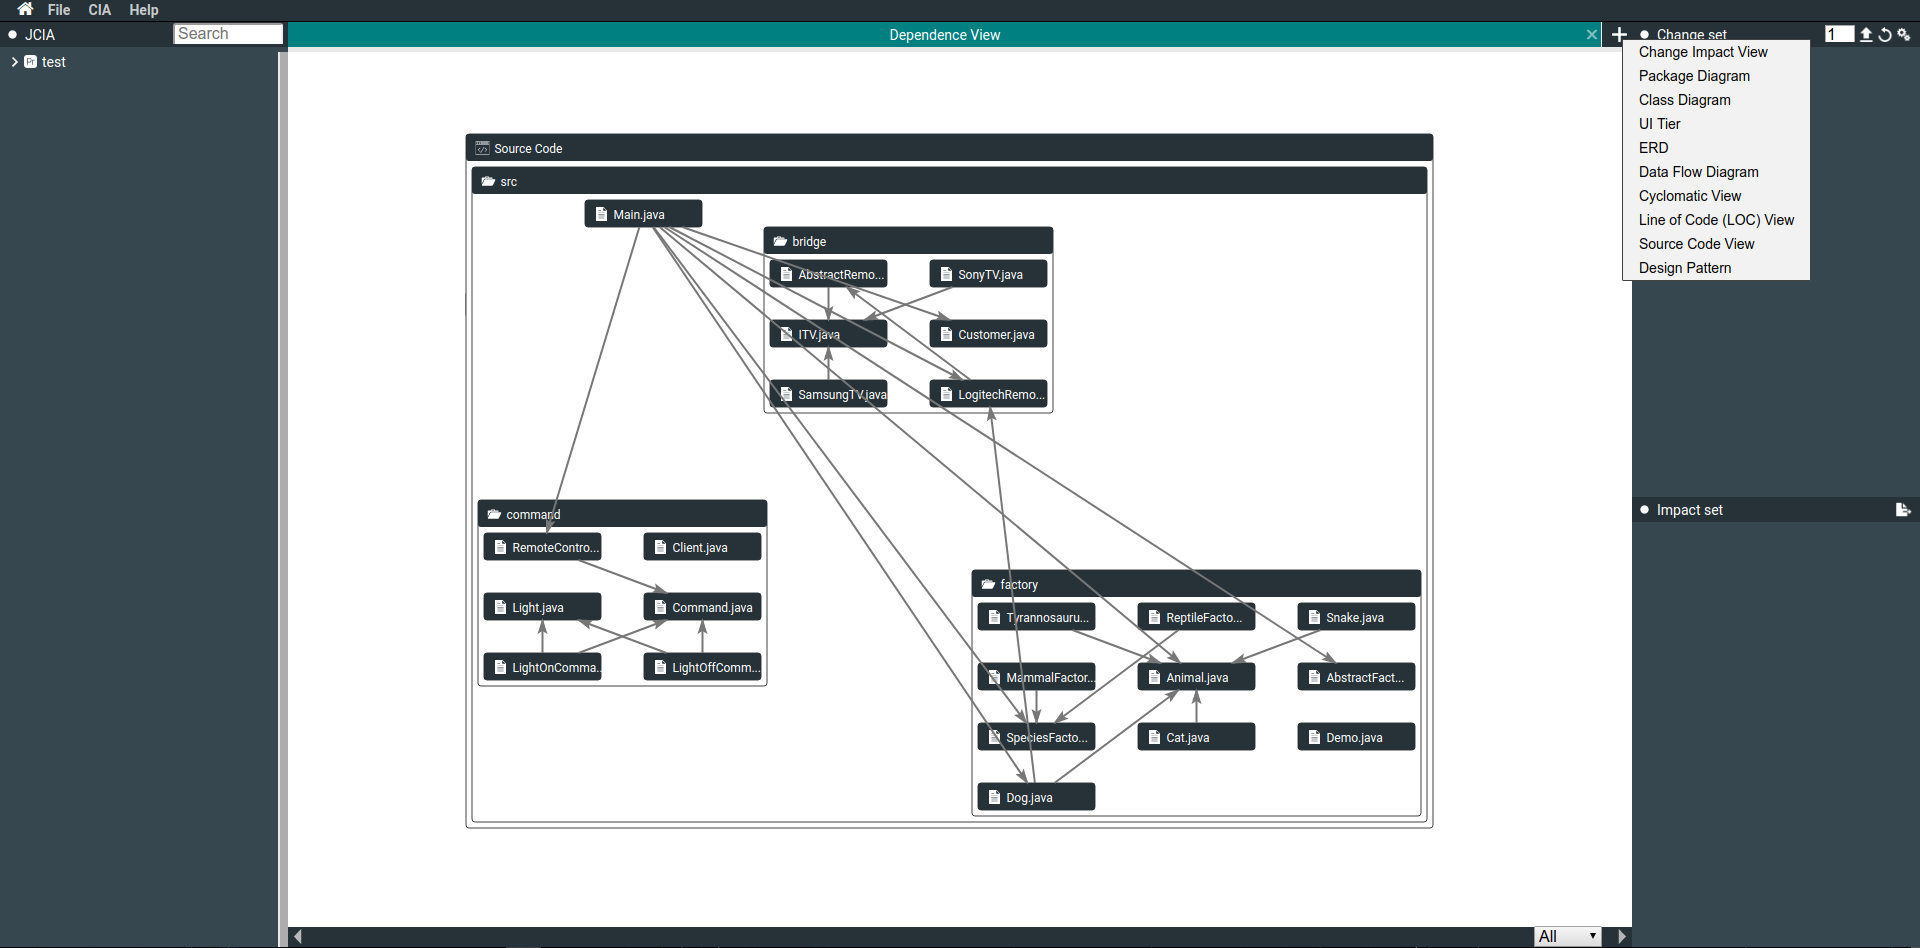
\includegraphics[scale=0.25]{images/main_screen}
	\caption{Giao diện chính và danh sách tính năng của JCIA-VT}
	\label{fig:main_screen}
\end{figure}\\
Mỗi màn hình đại diện cho một tính năng \textit{Dependency view} là mành hình mặc định trong giao diện làm việc, những màn hình làm việc còn lại được cung cấp tại danh mục tùy chọn, thể hiện như trong Hình \ref{fig:main_screen}

\noindent Tiếp theo, từ màn hình chính tại danh mục tình năng, ta lựa chọn \textit{Design Pattern} để chuyển tới màn hình làm việc của tính năng \textit{Kiểm tra sự tuân thủ mẫu thiết kế bên trong mã nguồn}. Hình \ref{fig:design_pattern_workspace} mô tả màn hình làm việc của tính năng \textit{Kiểm tra sự tuân thủ mẫu thiết kế}
\begin{figure}[h]i
	\centering
	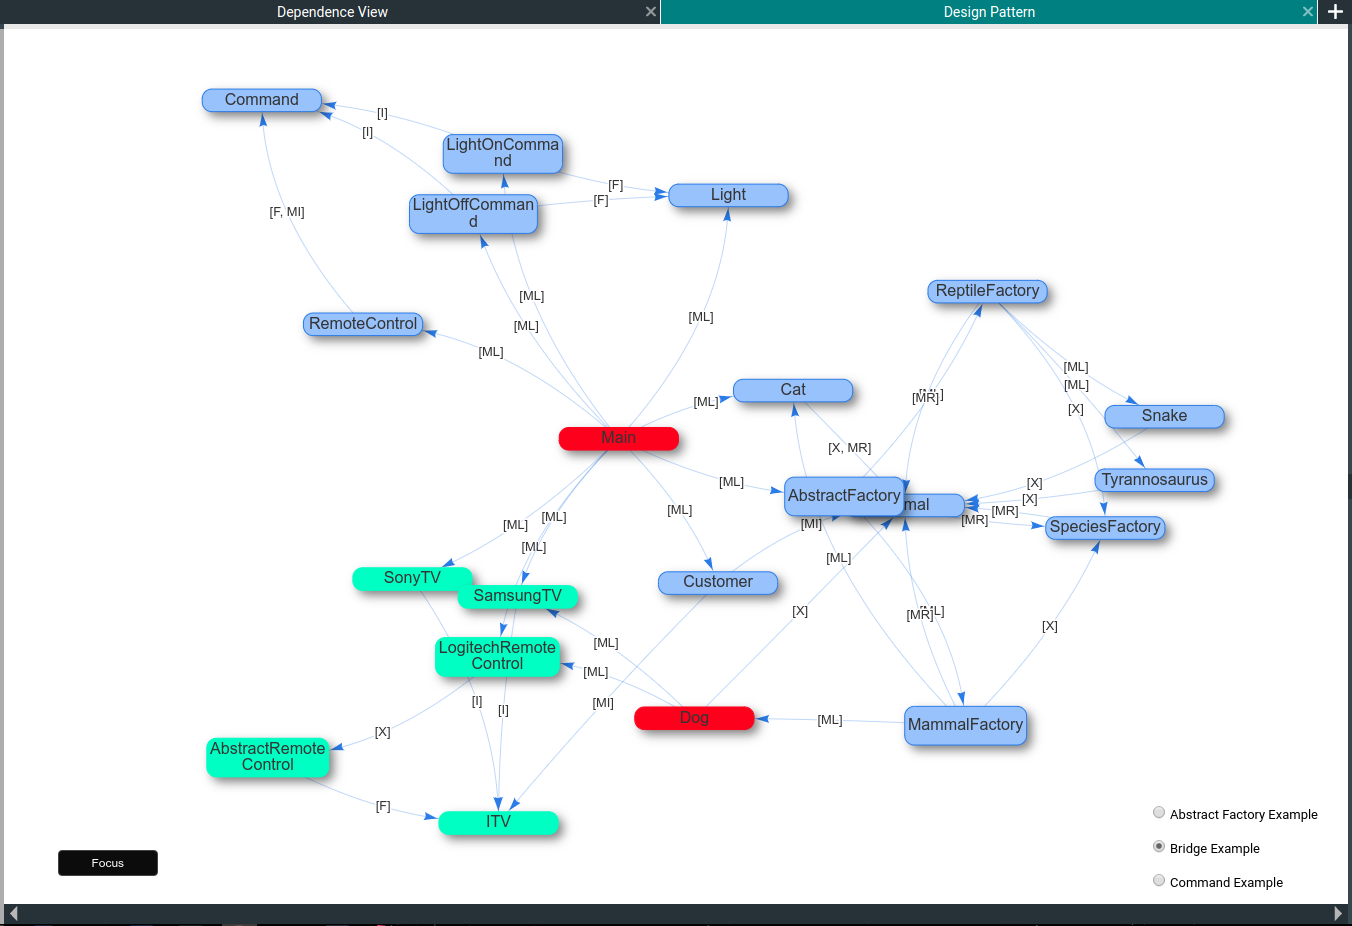
\includegraphics[scale=0.34]{images/design_pattern_workspace}
	\caption{Màn hình tính năng kiểm tra sự tuân thủ mã nguồn}
	\label{fig:design_pattern_workspace}
\end{figure}\\
Bao gồm, danh sách mẫu thiết kế được sử dụng trong mã nguồn dự án mà công cụ phát hiện được, đồ thị phụ thuộc của mã nguồn dự án. Trong đó, phần màu xanh của đồ thị là phần của một mẫu thiết kế mà công cụ phát hiện mã nguồn có sử dụng mẫu thiết kế đó, phần màu đỏ thể hiện phần mã nguồn liên quan tới mẫu thiết kế đó, tức là khi mau thiết kế thay đổi thì sẽ ảnh hưởng tới phần mã nguồn màu đỏ
\section{Thực nghiệm}
Trong phần này của khóa luận, sẽ tiến hành thực nghiệm công cụ đã được xây dựng. Tập dữ liệu thử nghiệm bao gồm mã nguồn có áp dụng những mẫu thiết kế hướng đối tượng được sử dụng phổ biết như Abstract Factory, Composite, Bridge, Adapter, Proxy v.v.
\noindent Ta sẽ trình bày một số ví dụ đã được sử dụng để tiến hành thực nghiệm trong quá trình xây dựng công cụ.

\noindent \textbf{Ví dụ 1}: Ví dụ này sẽ tiến hành thực nghiệm dựa trên một đoạn mã nguồn sử dụng Java đã được yêu cầu sử dụng ba mẫu thiết kế là Abstract Factory, Bridge, Command trong quá trình phát triển dự án. Hình \ref{fig:abstract_factory_diagram} mô tả biểu đồ lớp của mẫu Abstract Factory mà ta sẽ cần áp dụng trong mã nguồn ứng dụng.
\begin{figure}[h]
	\centering
	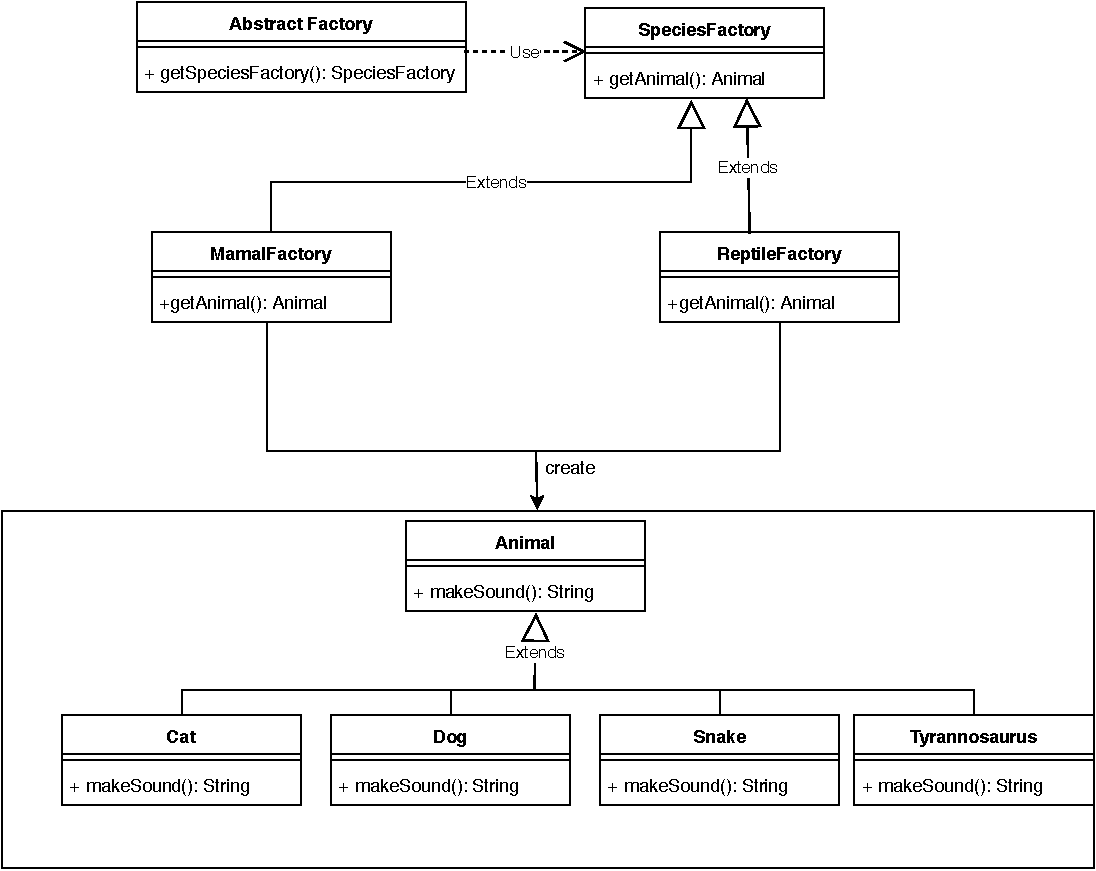
\includegraphics[scale=0.8]{images/_abstract_factory.pdf}
	\caption{Abstract Factory Class Diagram cho ví dụ 1}
	\label{fig:abstract_factory_diagram}
\end{figure}\\
\noindent \textbf{Điều kiện ban đầu}: Mã nguồn được yêu cầu áp dụng ba mẫu thiết kế là Abstract Factorym Bridge, Command.

\noindent \textbf{Các bước thực hiện}:\\
\texttt{Bước 1}: Triển khai (Implement) ba mẫu thiết kế và thực hiện tải lên JCIA-VT\\
\texttt{Bước 2}: Áp dụng ba mẫu thiết kế vào đoạn mã nguồn sẽ viết, sau đó phân tích đoạn mã nguồn đó với JCIA-VT để kiểm tra sự tuân thủ mẫu thiết kế.\\
\noindent \textbf{Kết quả mong đợi}: Công cụ sẽ kiểm tra sự tuân thủ mẫu thiết kế trong mã nguồn ứng dụng, phát hiện được ba mẫu thiết kế đã được áp dụng.\\\\\\\\\
\textbf{Thực hiện:}\\
\noindent \textbf{Bước 1}: Triển khai ba mẫu thiết kế. Hình \ref{fig:abstract_factory_diagram} mô tả cấu trúc của kiểu mẫu thiết kế Abstrac Factory. Ta sẽ viết mã Java triển khai lại mẫu thiết kế như trong biểu đồ lớp Hình \ref{fig:abstract_factory_diagram}. Thực hiện như vậy với cả ba mẫu thiết kê, sau đó tải chúng lên cơ sở dữ liệu mẫu thiết kế của bộ công cụ JCIA-VT, mỗi dự án sẽ có những bộ mẫu thiết kế khác nhau.\\\\
\noindent \textbf{Bước 2}: Sau khi áp dụng ba mẫu thiết kế kể trên vào trong mã nguồn, tiến hành phân tích mã nguồn bằng JCIA-VT, để kiểm tra sự tồn tại của những mẫu thiết kế đó trong mã nguồn và những mẫu thiết kế đó sẽ ảnh hưởng tới những thành phần nào trong mã nguồn. Từ đó ta sẽ đưa ra được kết luật về sự tuân thủ mẫu thiết kế bên trong mã nguồn.\\\\
\noindent \textbf{Kết quả}: Sau khi tiến hành phân tích, ta nhận được kết quả tra ra như Hình 4.9. Trong đó, màn hình thể hiện đã phát hiện được ba mẫu thiết được áp dụng trong mã nguồn. Đoạn đồ thị màu xanh non thể hiện thành phần chính của mẫu thiết kế (Bridge), tức là đây là thành phần đẳng cấu của mã nguồn với mẫu thiết kế (Bridge) mà công cụ phát hiện được. Phần đồ thị màu đỏ, thể hiện những thành phần mã nguồn có phụ thuộc với mẫu thiết kế đó trong mã nguồn.
\begin{figure}[h]
	\centering
	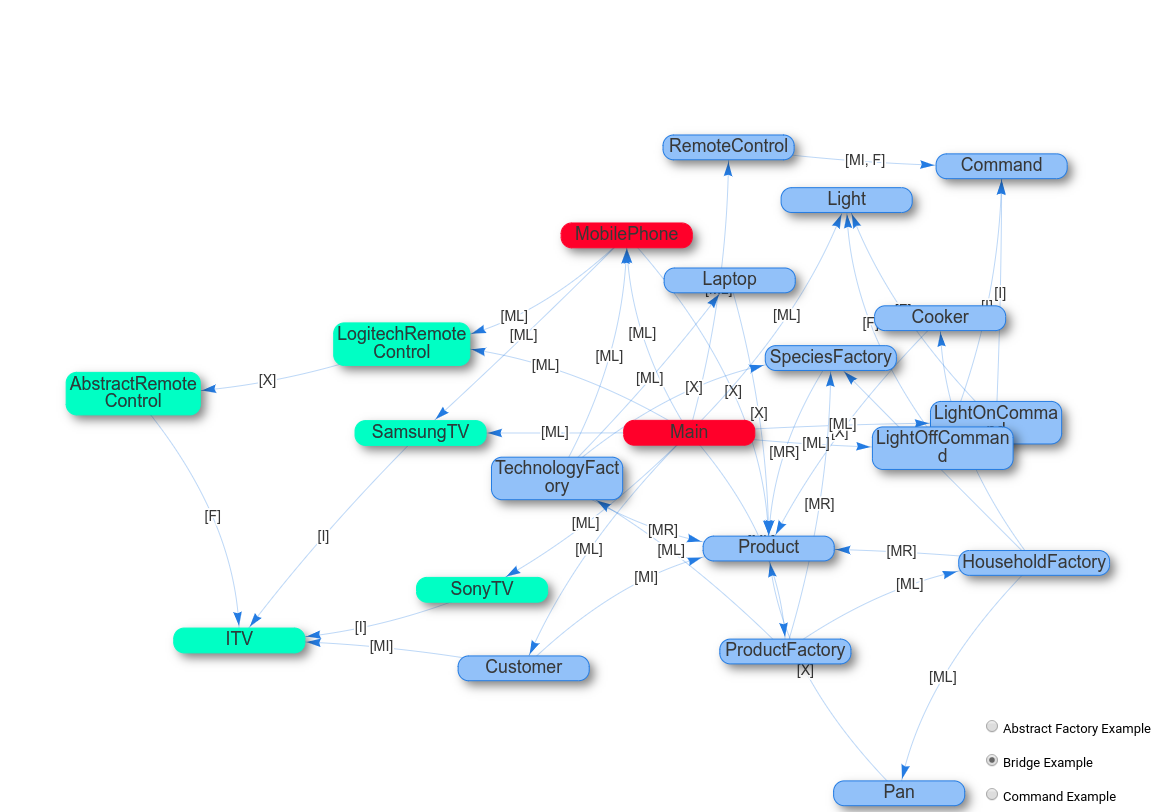
\includegraphics[scale=0.4]{images/result_example_1}
	\label{fig:result_example_1}
	\caption{Kết quả phân tích ví dụ 1}
\end{figure}\\
\newpage
\noindent \textbf{Ví dụ 2}: Sẽ thực hiện với kịch bản tương tự tại ví dụ 1, nhưng tại mã nguồn cần áp dụng mẫu Abstract Factory, ta đã áp dụng mẫu này khác so với mẫu Abstract Factory đã được tải lên cơ sở dữ liệu mẫu thiết kế của JCIA-VT. Tức là, về tính chất thì mã nguồn đã áp dụng đúng tính chất của mẫu Abstract Factory nhưng về mặt cấu trúc mã nguồn do khác so với cấu trúc mã nguồn đã tải lên cơ sở dữ liệu của JCIA-VT do vậy, công cụ sẽ không phát hiện được

\noindent \textbf{Điều kiện ban đầu}: Mã nguồn được yêu cầu áp dụng ba mẫu thiết kế là Abstract Factory, Bridge, Command. Trong đó mẫu Abstract Factory được áp dụng trong mã nguồn sẽ có cấu trúc khác với mẫu Abstract factory được yêu cầu như Hình \ref{fig:abstract_factory_diagram}. Hình \ref{fig:abstract_factory_diaram_2} là thể hiện cấu trúc mẫu Abstract Factory sẽ được áp dụng trong mã nguồn.
\begin{figure}[h]
	\centering
	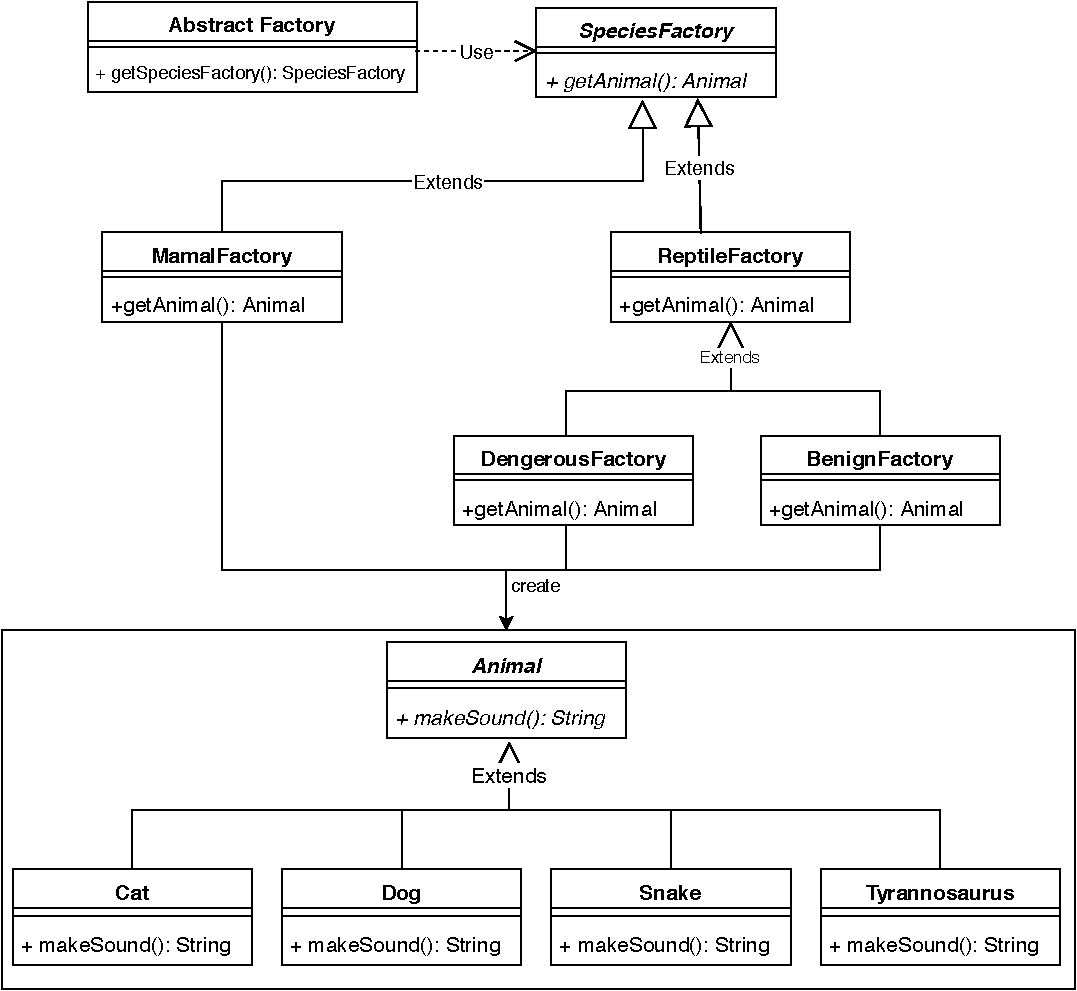
\includegraphics[scale=.8]{images/_abstract_factory_2.pdf}
	\label{fig:abstract_factory_diaram_2}
	\caption{Abstract Factory Diagram cho ví dụ 2}
\end{figure}

\noindent \textbf{Các bước thực hiện}: Các bước thực hiện sẽ tương tự như ví dụ 1 

\noindent \textbf{Kết quả}: Mẫu thiết kế Abstrac Factory sẽ không được phát hiện bởi công cụ.

\noindent \textbf{Lý giải}: Bản chất của việc phát hiện sự tuân thủ mẫu thiết kế là tiền hành kiểm tra mã nguồn có tồn tại những mẫu thiết kế như tài liệu đặc tả và thiết kế hay không. Phương pháp mà khóa luận này đề xuất tiếp cận theo hướng đồ thị. Tức là, ta có đồ thị phụ thuộc của mẫu thiết kế đã được triển khai trước đó và đồ thị phụ thuộc của toàn bộ mã nguồn ứng dụng. Công việc cần làm đó là tiến hành kiểm tra trong mã nguồn có tồn tại một đồ thị đẳng cấu với đồ thị của mẫu thiết kế hay không.
Do vậy triển khai mẫu thiết kế ban đầu là quan trọng sao cho mẫu thiết kế đó là đúng và gọn gàng nhất, khi áp dụng mẫu thiết kế đó vào mã nguồn đảm bảo rằngó trong mã nguồn ứng dụng mẫu thiết kế đo chỉ có xu hướng mở rộng so với định nghĩa ban đầu.

\noindent Trên đây là hai trong số nhiều ví dụ đã được thực hiện để kiểm tra tính đúng đắn của công cụ. Về cơ bản, công cụ hoạt động tốt với một số mẫu thiết kế thuộc \textit{GoF (Gang of Fours) design patters} \cite{go4} như Abstract Factory, Builder, Command,... bên cạnh đó còn gặp một số hạn chế về trùng lặp giữa các mẫu thiết kế.
Ngoài ra, công cụ còn hỗ trợ kiểm tra những mẫu thiết kế mà đội dự án tự định nghĩa. 

\subsection{Thảo luận}
Công cụ kiểm tra sự tuân thủ mẫu thiết kế do dự án sử dụng JAVA trong bộ công cụ JCIA-VT là một giải pháp cho việc đảm bảo chất lượng mã nguồn. Qua thực nghiệm, đã cho thấy tiềm năng của phương pháp mà khóa luận đề xuất.

\noindent Với ưu thế là phát triển công cụ trên nền tảng Web cho phép người dùng sẻ dụng nay trên những trình duyệt Web mà không phải cài đặt thêm bất chứ thứ gì. Điều này thúc đẩy khả năng tiếp cận của công cụ tới người dùng.

\noindent Đối với những dự án phần mềm, việc nắm bắt về thiết kế trong mã nguồn là rất cần thiết. Với sự ra đời của công cụ mà khóa luận này xây dựng, sẽ đem lại sự trợ giúp đắc lực trong các dự án phần mềm.

\noindent Qua thực nghiệm, ta thấy công cụ hoạt động tốt với những mẫu thiết kế do doanh nghiệp tự định nghĩa, một số những mẫu thiết kế cơ bản thuộc \textit{GoF (Gang of Fours) design patters} \cite{go4}. Bên cạnh đó, do thời gian là có hạn, tập phụ thuộc cần được đúc kết và nghiên cứu trong thời gian dài do vậy sự chưa đầy đủ về việc xác định phụ thuộc là không thể tránh khỏi, điều này dẫn tới trong thực nghiệm vẫn còn một số hạn chế về sự trùng lặp giữa các mẫu thiết kế, một số mẫu thiết kế chưa thể được phát hiện.

\noindent Những hạn chế này sẽ được khác phục liên tục trong những giai đoạn tiếp theo. Thực nghiệm cũng sẽ được thực hiện lại nhiều lần. Mục tiêu nhằm đem lại độ chính xác tốt hơn cho công cụ và trong tương lại công cụ có thể được đưa vào áp dụng trong thực tế tại các doanh nghiệp. Hiện tại công cụ đang nhận được một số phản hồi tích cự từ phía các chuyên gia tại Trung tâm Công nghệ và Quản lý chất lượng phần mềm Viettel.

\chapter{Kết luận}
Khóa luận này đã đề xuất phương pháp và xây dựng công cụ kiểm tra sự tuân thủ mẫu thiết kế của các dự án sử dụng Java. Ở giai đoạn này, khóa luận đã hoàn thành cơ bản các chức năng chính của công cụ. Phương pháp sẽ xây dựng một luồng xử lý mã nguồn Java, mã nguồn sẽ được phân tích thành cây cấu trúc, từ cây cấu trúc sẽ được tiếp tục phân tích để tìm những phụ thuộc tồn tại giữa hai thành phần mã nguồn, sau đó tiền hanh xây dựng đồ thị phụ thuộc từ mã nguồn. Mỗi khi người dùng muốn kiểm tra sự tuân thủ của mẫu thiết kế theo đặc tả của dự án, chỉ cần tải lên cơ sở dư liệu mẫu thiết kế của JCIA-VT những mẫu thiết kế mà mã nguồn sẽ áp dung theo như đặc tả ban đầu, sau đó tiến hành hành tải lên mã nguồn dự để phát hiện sự tuân thủ mẫu thiết kế của mã nguồn dự án đối với đặc tả ban đầu.

\noindent Bên cạnh đó, tiến hành tích hợp công cụ vào bộ công cụ đảm bảo chất lượng phần mềm JCIA-VT. Người dùng đã có thể tiến hành phân tích dự án, phát hiện sự tuân thủ mẫu thiết kê bên trong mã nguồn, không chỉ là những mẫu thiết kế phổ biến đã được định nghĩa sẵn mà còn hỗ trợ những mẫu thiết kế đặc thù ở từng doanh nghiệp khác nhau. Cùng hợp cùng với tiện ích quản lý phiên bản đã có của bộ JCIA-VT. Đem lại một tập các tiện ích phục vụ cho hoạt động quản lý phiên bản mã nguồn.

\noindent Dựa trên những gì đã thực hiện được của khóa luận này. Mặc dù công cụ còn còn tồn tại nhiều hạn chế và tính ứng dụng thực tế chưa cao. Tuy nhiên đã đem lại một nền tảng tốt, có thể tiếp tục hoàn thiện. Do đó, ở giai đoạn tiếp theo, phụ thuộc giữa các thành phần mã nguồn sẽ được tiếp tục nghiên cứu và thêm vào bộ phân tích của công cụ, nhằm cải thiện độ tin cậy của công cụ cũng như tăng khả năng áp dụng vào thực tế. Ngòai ra, tiếp tục phát triển thêm tính năng phát hiện thành phần mã nguồn áp dụng sai mẫu thiết kế nhằm tăng tính toàn diện của công cụ.
\begin{thebibliography}{9}
	\bibitem{jcia-vt}
	A Toolchain for Source Code Quality Assurance of Java EE Applications
	Bui, Quang Cuong and Dinh, Tien Loc and Luu, Anh Viet and Nguyen, Viet Hoa and Pham, Ngoc Quy and Pham, Ngoc Hung (2018) A Toolchain for Source Code Quality Assurance of Java EE Applications. Technical Report. Vietnam National University Hanoi
	
	\bibitem{orucc2016}
	 Murat Oruc, Fuat Akal, Hayri Server. Detecting Design Patterns in  Object-Oriented Design Models By Using Graph Mining Approach. pp 115,2016
	
	\bibitem{jcia}
	Ba Cuong Le, Son Nguyen Van, Duc Anh Nguyen, Ngoc Hung Pham, Hieu Vo Dinh. JCIA: A Tool for Change Impact Analysis of Java EE Applications. Information Systems Design and Intelligent Applications, pp.105-114, 2018.
	
	\bibitem{jp}
	Nicholas Smith, Danny van Bruggen, Federico Tomassetti
	JavaParser: Visited
	Analyse, transform and generate your Java code base
	
	\bibitem{vf2}
	Luigi P. Cordella, Pasquale Foggia, Carlo Sansone,and Mario Vento. A (Sub)Graph Isomorphism Algorithm for
	Matching Large Graphs 10-2004 P1367
	
	\bibitem{vf2_1368}
	Luigi P. Cordella, Pasquale Foggia, Carlo Sansone,and Mario Vento. A (Sub)Graph Isomorphism Algorithm for
	Matching Large Graphs 10-2004 P1368-1369
	
	\bibitem{go4}
	Design Patterns: Elements of Reusable Object-Oriented Software by ErichGamma, RichardHelm, RalphJohnson, and JohnVlissides (the GangOfFour)
\end{thebibliography}
\end{document}
